\newpage
\appendix
\onecolumn

% \section{Multiple agents}
% The action space $\mathcal{A}^r$ is defined as $\mathcal{A}^r = \{$\texttt{[No Retrieval]},\texttt{[Retrieval]<query>}, \texttt{[Planning]}$\}$, where \texttt{<query>} represents the space of possible queries.


% The action space $\mathcal{A}^d$ is defined as $\mathcal{A}^d = \{\texttt{Retrieval} \times \mathcal{Q}\} \cup \{\texttt{LLM}\}$, where $\mathcal{Q}$ represents the space of possible subqueries.

% \section{Discussions}

% \subsection{Future Work}

% \subsection{Limitations}
% sft warm-up  from zero

\section{More Implementation Details}\label{app:imple_details}

In this section, we provide a comprehensive implementation details of our proposed method. For additional insights and more intricate details, we refer the reader to our supplementary materials.


\subsection{RL Training Process}\label{app:ppo_details}
Having obtained the credit rewards that reflect each agent's contribution, we develop an optimization framework to guide end-to-end training across all agents. % encourage collaborative behaviors among agents
The key idea is to use these credit signals for optimizing the collaborative behavior of the entire system.
The optimization objective for our multi-agent system can be formulated as maximizing the expected credit rewards:
\begin{equation}
    \mathcal{J}(\theta) = \mathbb{E}_{\tau \sim \pi_\theta}\left[\sum_{i\in \mathcal{N}}\sum_{t} r_{\text{credit}}(s^i_t, a^i_t)\right]
\end{equation}
% We optimize this objective using Proximal Policy Optimization (PPO)~\citep{SchulmanWDRK17}.
% Since each agent's action is a sequence of tokens, we optimize this objective using Proximal Policy Optimization (PPO)~\citep{SchulmanWDRK17} and decompose the optimization at the token level~\citep{Ouyang0JAWMZASR22}. Specifically, we define:
Since each agent's action is a sequence of tokens, we decompose this optimization using Proximal Policy Optimization (PPO)~\citep{SchulmanWDRK17,abs-2312-01058,ZhuDW24} as follows:
\begin{equation}
    \mathcal{L}_{\text{\modelname}} = \sum_{i\in\mathcal{N}} \mathcal{L}_{\text{PPO}}^i(\theta, \phi)
\end{equation}
Specifically, for each agent $i$, we define:
\begin{equation}
    \mathcal{L}_{\text{CLIP}}^i(\theta)
    = \mathbb{E}_{\tau \sim \pi_\theta}\Big[\sum_{t}\sum_{m} \min\big(r_{t,m}^i(\theta)\hat{A}_{t,m}^i, \text{clip}(r_{t,m}^i(\theta), 1-\epsilon, 1+\epsilon)\hat{A}_{t,m}^i\big)\Big]
\end{equation}
% \begin{equation}
%     \mathcal{L}_{\text{CLIP}}(\theta)
%     = \mathbb{E}_{\tau \sim \pi_\theta}\Big[\sum_{i\in \mathcal{N}}\sum_{t}\sum_{m} \min\big(r_{t,m}^i(\theta)\hat{A}_{t,m}^i, \text{clip}(r_{t,m}^i(\theta), 1-\epsilon, 1+\epsilon)\hat{A}_{t,m}^i\big)\Big]
% \end{equation}
where $r_{t,m}^i(\theta) = \frac{\pi_\theta(a_{t,m}^i|s_{t,m}^i)}{\pi_{\theta_{\text{old}}}(a_{t,m}^i|s_{t,m}^i)}$ is the probability ratio, $s_{t,m}^i$ represents the concatenation of current state and the first $m-1$ tokens in the action sequence for agent $i$ at time step $t$, and $a_{t,m}^i$ denotes its $m$-th token.
We compute the advantage estimate using GAE~\citep{SchulmanMLJA15}: $\hat{A}_{t,m}^i = \sum_{l=0}^{M-m-1}(\gamma\lambda)^l\delta_{t,m+l}^i$, where $M$ is the token length of the action sequence.
% We compute the advantage estimate using GAE~\citep{SchulmanMLJA15}: $\hat{A}_{t,m}^i = \sum_{l=0}^{M-m-1}(\gamma\lambda)^l\delta_{t,m+l}^i$, where $M$ is the token length of the action sequence, and $\delta_{t,m}^i = r_{\text{token}}(s_{t,m}^i, a_{t,m}^i) + \gamma V_\phi(s_{t,m+1}^i) - V_\phi(s_{t,m}^i)$ is the TD-error.
% The advantage estimate $\hat{A}_{t,m}^i$ is computed using Generalized Advantage Estimation (GAE):
% \begin{equation}
%     \hat{A}_{t,m}^i = \delta_{t,m}^i + (\gamma\lambda)\delta_{t,m+1}^i + ... + (\gamma\lambda)^{M-m+1}\delta_{t,M-1}^i
% \end{equation}
% where $M$ is the token length of the corresponding response sequence, and $\delta_{t,m}^i = r_{\text{token}}(s_{t,m}^i, a_{t,m}^i) + \gamma V_\phi(s_{t,m+1}^i) - V_\phi(s_{t,m}^i)$ is the TD-error.
% The token-level reward $r_{\text{token}}$ incorporates both the tree credit and a KL penalty term:
% \begin{equation}
%     r_{\text{token}}(s_{t,m}^i, a_{t,m}^i) = \begin{cases}
%         r_{\text{credit}}(s_t^i, a_t^i) -\beta \text{KL}(m) & m = M \\
%         -\beta \text{KL}(m) & \text{otherwise}
%     \end{cases}
% \end{equation}
% where $\text{KL}(m) = \log \frac{\pi_{\theta_{\text{old}}}(a_{t,m}^i|s_{t,m}^i)}{\pi_{\theta_{\text{ref}}}(a_{t,m}^i|s_{t,m}^i)}$, and $\beta$ is a hyperparameter that controls the strength of the KL penalty.

To estimate state values across the multi-agent system, we employ a centralized state-value function $V_\phi$ that takes each agent's state $s_{t,m}^i$ as input. The value function is optimized to minimize the mean squared error~\citep{LoweWTHAM17}:
\begin{equation}
    \mathcal{L}_V^i(\phi) = \mathbb{E}_{\tau \sim \pi_\theta}\left[\sum_{t}\sum_{m} (V_\phi(s_{t,m}^i) - \hat{G}_{t,m}^i)^2\right]
\end{equation}
where $\hat{G}_{t,m}^i = \hat{A}_{t,m}^i + V_\phi(s_{t,m}^i)$ is the empirical return.
The final optimization objective combines the policy and value losses:
\begin{equation}
    \mathcal{L}_{\text{PPO}}^{i}(\theta, \phi) = \mathcal{L}_{\text{CLIP}}^{i}(\theta) + c_v \mathcal{L}_V^i(\phi)
\end{equation}
where $c_v$ controls the weight of the value loss. This joint objective enables end-to-end training of both policy and value networks across all agents.
% Therefore, for multi-agent reinforcement learning~\citep{abs-2312-01058,ZhuDW24}, we have the final training objective:
% \begin{align}
%     \mathcal{L}_{\text{\modelname}} &= \sum_{i\in\mathcal{N}} \mathcal{L}_{\text{PPO}}^i(\theta, \phi) \nonumber \\
%     &= sum_{i\in\mathcal{N}} \Big(
%         \mathcal{L}_{\text{CLIP}}^{i}(\theta) + c_v \mathcal{L}_V^i(\phi)
%     \Big)
%     &= \sum_{i\in \mathcal{N}} \Big( \mathbb{E}_{\tau \sim \pi_\theta}\Big[\sum_{t}\sum_{m} \min\big(r_{t,m}^i(\theta)\hat{A}_{t,m}^i, \text{clip}(r_{t,m}^i(\theta), 1-\epsilon, 1+\epsilon)\hat{A}_{t,m}^i\big)\Big]
%     + \nonumber \\
%     &\mathbb{E}_{\tau \sim \pi_\theta}\left[\sum_{t}\sum_{m} (V_\phi(s_{t,m}^i) - \hat{G}_{t,m}^i)^2\right] \nonumber \\
%     &= \mathbb{E}_{\tau \sim \pi_\theta}\Big[\sum_{i\in \mathcal{N}}\sum_{t}\sum_{m} \min\big(r_{t,m}^i(\theta)\hat{A}_{t,m}^i, \text{clip}(r_{t,m}^i(\theta), 1-\epsilon, 1+\epsilon)\hat{A}_{t,m}^i\big)\Big]
% \end{align}


% In cooperative multi-agent system, we employ a centralized state-value function $V_\phi$ shared across all agents to estimate the value of each agent's state $s_{t,m}^i$. This value function is optimized to minimize the mean squared error between its predictions and the empirical returns across all agents:
% \begin{equation}
%     L_V(\phi) = \mathbb{E}_{\tau \sim \pi_\theta}\left[\sum_{i\in \mathcal{N}}\sum_{t}\sum_{m} (V_\phi(s_{t,m}^i) - \hat{G}_{t,m}^i)^2\right]
% \end{equation}
% where $\hat{G}_{t,m}^i = \hat{A}_{t,m}^i + V_\phi(s_{t,m}^i)$ is the empirical return.
% The final optimization objective combines the policy and value losses:
% \begin{equation}
%     L(\theta, \phi) = L^{\text{CLIP}}(\theta) - c_v L_V(\phi)
% \end{equation}
% where $c_v$ is a coefficient for the value loss.
% This overall optimization is performed in an end-to-end manner across all agents simultaneously.


\subsection{Implementation Details}
\textbf{Supervised Warm-up Phase:} 
We utilize \texttt{Llama-Factory}~\citep{zheng2024llamafactory} as our training framework for the initial supervised fine-tuning phase. The detailed hyper-parameters for this phase are presented in Table~\ref{tab:sft_params}.
\begin{table}[h]
\centering
\caption{Key hyperparameters in the supervised warm-up phase.}
\label{tab:sft_params} 
% \resizebox{0.99\linewidth}{!}{
% \begin{small}
\begin{tabular}{@{}lc@{}}
\toprule
\textbf{Hyperparameter} & \textbf{Value}                         \\ \midrule
Learning Rate           & 4e-5                                   \\
Batch size              & 512                                    \\
\#Epochs                & 3                                      \\
Optimizer type          & AdamW~\citep{LoshchilovH19}            \\
Chat template           & \texttt{Qwen}~\citep{qwen2}            \\
Base model              & Qwen2-1.5B or Qwen2-0.5B~\citep{qwen2} \\
Cutoff length           & 4096                                   \\
Warmup ratio            & 0.03                                   \\
LR scheduler type       & Cosine                                 \\ \bottomrule
\end{tabular}
% }
% \end{small}
\end{table}

\textbf{Reinforcement Learning Phase:} 
For the RL training phase, we adopt \texttt{OpenRLHF}~\citep{hu2024openrlhf} as our primary training framework, coupled with \texttt{VLLM}~\citep{kwon2023efficient} inference engine. The complete set of RL training hyper-parameters is detailed in Table~\ref{tab:rl_params}. To initialize both the policy and value models, we leverage the model obtained after one epoch of supervised fine-tuning, with the language model head replaced by a value head for the value model.
\begin{table}[h]
\centering
\caption{Key hyperparameters in the RL phase.}
\label{tab:rl_params} 
% \resizebox{0.99\linewidth}{!}{
% \begin{small}
\begin{tabular}{@{}lc@{}}
\toprule
\textbf{Hyperparameter}       & \textbf{Value} \\ \midrule
Learning Rate of Policy model & 5e-7           \\
Learning Rate of Value model  & 5e-6           \\
Batch size                    & 1024           \\
KL Coefficient                & 0.005          \\
Optimizer type                & Adam           \\
Prompt max len                & 4096           \\
Generate max len              & 2048           \\
Maximal depth                 & 13             \\
LR scheduler type             & Cosine         \\ \bottomrule
\end{tabular}
% }
% \end{small}
\end{table}

% \textbf{Inference Phase\footnote{We have released all the code in the Supplementary Material.}:}
% We construct our retrieval server using the 2018 Wikipedia dump~\citep{yang-etal-2018-hotpotqa} as the knowledge source and use contriever-msmarco~\citep{IzacardCHRBJG22} as our dense retriever.
% We also adopt the \href{https://docs.sglang.ai/}{\texttt{SGLang}}\footnote{\url{https://docs.sglang.ai/}} as the LLM server to support different model, such as Qwen2-72B-Instruct~\citep{qwen2}, Llama3.3-70B-Instruct~\citep{llama3}.
% Our inference code support two efficient inference engine: \texttt{SGLang} and \texttt{VLLM}.

\textbf{Inference Phase\footnote{The complete implementation code is available in the Supplementary Material.}:}
For the deployment of our system, we establish a comprehensive infrastructure that integrates multiple components:

\begin{itemize}[topsep=1pt, partopsep=1pt, leftmargin=12pt, itemsep=-1pt]
    \item \textbf{Retriever Server:} We construct our retrieval server using the 2018 Wikipedia dump~\citep{yang-etal-2018-hotpotqa} as the primary knowledge source. We employ contriever-msmarco~\citep{IzacardCHRBJG22} as our dense retriever for efficient and effective document retrieval. Our inference code also supports Google search engine~\citep{schmidt2014google} as the retriever server.
    
    \item \textbf{LLM Service:} We integrate \href{https://docs.sglang.ai/}{\texttt{SGLang}}\footnote{\url{https://docs.sglang.ai/}} as our LLM server, which provides compatibility with various state-of-the-art language models, including Qwen2-72B-Instruct~\citep{qwen2} and Llama3.3-70B-Instruct~\citep{llama3}. Moreover, we also support GPT series models\footnote{We use \texttt{gpt-4o-mini-2024-07-18} in our out-of-generalization experiments.}.
    
    \item \textbf{Inference Optimization:} Our implementation supports two high-performance inference engines: \texttt{SGLang} and \texttt{VLLM}, allowing users to optimize for different deployment scenarios and hardware configurations.
\end{itemize}

This modular architecture ensures both flexibility in model selection and efficiency in deployment, while maintaining robust performance across different configurations.

% \textbf{Other Details in our \modelname.}


\subsection{Dataset Details}
\begin{table}[h]
\centering
\caption{Training Dataset Statistics.}
\label{tab:data_statistics} 
\resizebox{\linewidth}{!}{
% \begin{small}
\begin{tabular}{@{}l|ccc|ccc|c@{}}
\toprule
\multirow{2}{*}{\textbf{Data Name}} & \multicolumn{3}{c|}{\textbf{Multi-Hop}} & \multicolumn{3}{c|}{\textbf{Single-Hop}} & \multirow{2}{*}{\textbf{Total}} \\
                                    & 2WikiMultiHopQA  & HotpotQA  & Musique  & Natural Questions  & PopQA   & TriviaQA  &                                 \\ \midrule
\textbf{Raw Data Size}              & 167,454          & 90,447    & 19,938   & 79,169             & 12,868  & 78,785    & 448,661                         \\
\textbf{Our Train Data Size}        & 6,000            & 6,000     & 6,000    & 6,000              & 6,000   & 6,000     & 36,000                          \\
\textbf{Sampling ratio}             & 3.5\%            & 6.6\%     & 30.1\%   & 7.5\%              & 46.6\%  & 7.6\%     & 8.02\%                          \\ \bottomrule
\end{tabular}
}
% \end{small}
\end{table}
\textbf{In-domain Datasets.}
As shown in Table~\ref{tab:data_statistics}, we conduct extensive in-domain experiments on three single-hop and three multi-hop datasets.
For each dataset, we randomly sampled 6,000 instances as the training set, with sampling ratios detailed in Table~\ref{tab:data_statistics}. Overall, we utilize only 8\% of the original data as the training set.
For the in-domain test sets, we randomly sampled 1,000 instances as the test set.

\begin{table}[h]
\centering
\caption{Out-of-generalization Dataset Statistics.}
\label{tab:ood_statistics} 
% \resizebox{\linewidth}{!}{
% \begin{small}
\begin{tabular}{@{}lcc@{}}
\toprule
          & \textbf{FreshQA} & \textbf{Multihop-RAG} \\ \midrule
Data Size & 500              & 2556                  \\ \bottomrule
\end{tabular}
% }
% \end{small}
\end{table}

\textbf{Out-of-generalization Datasets.}
To comprehensively evaluate the plug-and-play capability of our \modelname in out-of-distribution generalization scenarios, we introduce two recent challenging datasets: FreshQA~\citep{VuI0CWWTSZLL24} and Multihop-RAG~\citep{multihop_rag}. 
The statistics of the OOD datasets are summarized in Table~\ref{tab:ood_statistics}.

% \subsection{Overall Algorithm}
% In this section, we present the inference process of \modelname for reference, as shown in the Algorithm~\ref{alg:infer_alg}.

% \begin{algorithm}[h]
    \caption{Inference Process of our \modelname}
    \label{alg:infer_alg}
    \begin{algorithmic}[1]
        \INPUT question $q$, the retrieval server (\textbf{Retriever}), the LLM server (\textbf{LLM}), the proxy model in our \modelname $\pi$, instruction for different agent (Reasoning Router, Information Filter, and Decision Maker).
        \OUTPUT The Answer.

        \STATE $a^1 \leftarrow \pi(q, \text{instruction}_1)$ \COMMENT{Reasoning Router agent}

        \IF{$a^1$==\texttt{[No Retrieval]}}
        \STATE $\text{Answer} \leftarrow \textbf{LLM}(q)$ \COMMENT{Direct Answering Strategy, \textcolor{red}{if $q$ does not require retrieval}}
        \ELSIF{$a^1$==\texttt{[Retrieval]<query content>}} 
        \STATE $\text{docs} \leftarrow \textbf{Retrieval}(\texttt{<query content>})$
        \STATE $\text{selected docs} (a^2) \leftarrow \pi(q, \text{docs}, \text{instruction}_2)$ \COMMENT{Information Filter agent}
        \STATE $\text{Answer} \leftarrow \textbf{LLM}(q, \text{selected docs})$ \COMMENT{Single-pass Strategy, \textcolor{red}{if $q$ requires retrieval and is simple question}}
        \ELSE
        \STATE Accumulated\_docs $\leftarrow \emptyset$ 
        \STATE $\text{Roadmap}\leftarrow \textbf{LLM}(q)$ \COMMENT{$a^1==\texttt{[Planning]}$}
        \STATE $a^3 \leftarrow \pi(q, \text{Roadmap}, \text{Accumulated\_docs}, \text{instruction}_3)$ \COMMENT{Decision Maker agent}
        \WHILE{$a^3 \neq \texttt{[LLM]}$ }
            \STATE $\text{docs} \leftarrow \textbf{Retrieval}(\texttt{<subquery content>}~\text{in}~a^3)$
            \STATE $\text{selected docs} (a^2) \leftarrow \pi(q, \text{docs}, \text{instruction}_2)$ \COMMENT{Information Filter agent}
            \STATE Accumulated\_docs $\leftarrow \{\text{Accumulated\_docs}\} \cup \{\text{selected docs}\}$ 
            \STATE $a^3 \leftarrow \pi(q, \text{Roadmap}, \text{Accumulated\_docs}, \text{instruction}_3)$ \COMMENT{Decision Maker agent}
        \ENDWHILE
        \STATE $\text{Answer} \leftarrow \textbf{LLM}(q, \text{Accumulated\_docs})$ \COMMENT{Multi-step Reasoning Strategy, \textcolor{red}{if $q$ requires retrieval and is complex}}
        \ENDIF
    \end{algorithmic}
\end{algorithm}


\section{Instructions and State Transition Function}\label{app:instructions}
\subsection{Instructions for Each Agent}
In this section, we details the state space and action space fo each agent in our \modelname.

\textbf{Reasoning Router.}
The Reasoning Router agent operates with state space $\mathcal{S}^1=\{q\}$, where $q$ represents the input question.
This agent is responsible for determining whether retrieval is necessary for the given question and assessing the question complexity when retrieval is needed.
For a question that does not require retrieval, this agent outputs \texttt{[No Retrieval]}.
If the retrieval is needed, the agent outputs one of the following actions based on the complexity of the question $q$: for simple questions requiring retrieval: \texttt{[Retrieval]<query content>}, initiating a single-pass retrieval-filter loop, where \texttt{<query content>} defines the space of possible queries;
for complex questions: \texttt{[Planning]}, triggering the multi-step reasoning strategy.
The specific examples are as follows:
\begin{tcolorbox}[title=Reasoning Router,width=\linewidth, breakable]
\begin{small}
\textcolor{red}{Instruction for Reasoning Router}\\
You are an intelligent assistant tasked with evaluating whether a given question requires further information through retrieval or needs planning to arrive at an accurate answer. You will have access to a large language model (LLM) for planning or answering the question and a retrieval system to provide relevant information about the query. \\

Instructions:\\
1. **Evaluate the Question**: Assess whether a precise answer can be provided based on the existing knowledge of LLM. Consider the specificity, complexity, and clarity of the question.\\
2. **Decision Categories:**\\
    - If the question is complex and requires a planning phase before retrieval, your response should be:\\
    \texttt{[Planning]}\\
    - If the question requests specific information that you believe the LLM does not possess or pertains to recent events or niche topics outside LLM's knowledge scope, format your response as follows: \\
    \texttt{[Retrieval] `YOUR QUERY HERE`}\\
    - If you think the LLM can answer the question without additional information, respond with:\\
    \texttt{[No Retrieval]}\\
3. **Focus on Assessment**: Avoid providing direct answers to the questions. Concentrate solely on determining the necessity for retrieval or planning.\\

\textcolor{red}{State of Reasoning Router}\\
Now, process the following question:\\
\\
Question: \{question\}\\

\textcolor{red}{Output (All possible Actions) of Reasoning Router}\\
\% For No Retrieval\\
\texttt{[No Retrieval]}\\
\% For Retrieval\\
\texttt{[Retrieval]<query content>} (for simple questions)\\
\texttt{[Planning]} (for complex questions)
\end{small}
\end{tcolorbox}


\textbf{Information Filter.}
The state space of Information Filter consists of the question $q$, the retrieved documents, and the current objective (if in \texttt{[Planning]} mode), i.e., $\mathcal{S}^2=\{q, \text{retrieved documents}\}$ for single-pass strategy (\texttt{Retrieval<query content}), or $\mathcal{S}^2=\{q, \text{retrieved documents}, \text{current objective}\}$ for multi-step reasoning strategy (\texttt{[Planning]}).
\begin{tcolorbox}[title=Information Filter,width=\linewidth, breakable]
\begin{small}
\textcolor{red}{Instruction for Information Filter}\\
You are an intelligent assistant tasked with analyzing the retrieved documents based on a given question and the current step's objectives. Your role is to determine the relevance of each document in relation to the question and the specified objectives.\\

Instructions:\\
1. **Analyze Relevance**: Evaluate each document whether it aligns with the objectives of the current retrieval step and contains a direct answer to the question.\\
2. **Thought Process**: Provide a brief analysis for each document, considering both the answer content and the retrieval objectives.\\
3. **Filter Documents**: After your thought process, generate a list of document indices indicating which documents to retain.\\

\textcolor{red}{State of Information Filter}\\
Now, process the following question:\\
\\
Current step's objectives: \{objective\} (only for \texttt{[Planning]} mode)\\

Question: \{question\}\\

Documents:
\{documents\}\\

\textcolor{red}{Output of Information Filter}\\
Thought: $<$Analysis of each documents$>$\\
Action: [$<$Selected document IDs$>$]
\end{small}
\end{tcolorbox}



\textbf{Decision Maker.}
The Decision Maker agent operates with state space $\mathcal{S}^3=\{q, \text{Accumulated Documents}, \text{Roadmap}\}$.
Based on the current state, this agent outputs one of two possible actions: \texttt{[Retrieval]<subquery content>} (requesting additional retrieval-filtering loop through the sub-query) or \texttt{[LLM]} (passing all accumulated documents to LLM for generating the final answer).
\begin{tcolorbox}[title=Decision Maker,width=\linewidth, breakable]
\begin{small}
\textcolor{red}{Instruction for Decision Maker}\\
You are an intelligent assistant tasked with determining the next appropriate action based on the provided existing documents, plan, and question. You have access to a large language model (LLM) for answering question and a retrieval system for gathering additional documents. Your objective is to decide whether to write a query for retrieving relevant documents or to generate a comprehensive answer using the LLM based on the existing documents and plan.\\

Instructions:\\
1. **Evaluate Existing Documents**: Assess the existing documents to determine if it is sufficient to answer the question.\\
2. **Follow the Plan**: Understand the next steps outlined in the plan.\\
3. **Decision Categories:**\\
    - If the existing documents is insufficient and requires additional retrieval, respond with:\\
        \texttt{[Retrieval] `YOUR QUERY HERE`}\\
    - If the existing documents is adequate to answer the question, respond with:\\
        \texttt{[LLM]}\\
4. **Focus on Action**: Do not answer the question directly; concentrate on identifying the next appropriate action based on the existing documents, plan, and question.\\

\textcolor{red}{State of Decision Maker}\\
Now, process the following question:\\
\\
Existing Documents: \{accumulated documents\}\\

Roadmap: \{roadmap\}\\

Question: \{question\}\\

\textcolor{red}{Output of Decision Maker}\\
Thought: {[}Your analysis for current situation (need retrieval for additional informations or use LLM to answer){]}\\
Action: {[}Your decision based on the analysis (\texttt{[Retrieval]<subquery content>} or \texttt{[LLM]}){]}
\end{small}
\end{tcolorbox}



\subsection{State Transition Function}\label{app:transition_details}
Given a state $s_t^i$ and an action $a_t^i$ in each agent $i\in \mathcal{N}$, the transition function $\mathcal{T}$ in our framework is deterministic.
Based on the three collaborative strategies introduced in Section~\ref{sec:strategy}, the state transitions are defined as follows:

\textbf{Direct Answering Strategy} (\texttt{[No Retrieval]}): In this strategy, the LLM directly generates the answer without retrieval, resulting in no state transitions between agents.

\textbf{Single-pass Strategy} (\texttt{[Retrieval]<query content>}): This strategy involves a state transition between the Reasoning Router and Information Filter agents:
\begin{equation}
    \mathcal{T}: \mathcal{S}^1=\{q\} \times \mathcal{A}=\{\texttt{[Retrieval]<query content>}\} \xrightarrow{\text{retrieval}} \mathcal{S}^2 = \{q, \text{retrieved documents}\}
\end{equation}
where $\mathcal{S}^1$ represents the initial state with the question $q$, and $\mathcal{S}^2$ represents the state for the Information Filter agent after retrieval. The Information Filter is responsible for filtering the helpful documents based on $\mathcal{S}^2$.


\textbf{Multi-Step Reasoning Strategy} (\texttt{[Planning]}): This strategy involves multiple state transitions in a cyclic manner:


\begin{itemize}[topsep=1pt, partopsep=1pt, leftmargin=12pt, itemsep=-1pt]
    \item Reasoning Router $\rightarrow$ Decision Maker: %Given the LLM-generated roadmap after \texttt{[Planning]}, we have the state $\mathcal{S}^3=\{q, \text{Accumulated Documents}, \text{Roadmap}\}$ in Decision Maker agent.
    \begin{equation}
        \mathcal{T}: \mathcal{S}^1=\{q\} \times \mathcal{A}=\{\texttt{[Planning]}\} \xrightarrow{\text{\texttt{[planning]}}} \mathcal{S}^3 = \{q, \text{Accumulated Documents}, \text{Roadmap}\},
    \end{equation}
    where the roadmap is generated by the LLM and the accumulated documents is empty for initial step.
    \item Decision Maker $\rightarrow$ Information Filter: %Given the current step's objective and retrieved documents based on the \texttt{[Retrieval]<subquery content>} outputted by the Decision Maker, we have the state $\mathcal{S}^2=\{q, \text{retrieved documents}, \text{current objective}\}$ in the Information Filter agent.
    \begin{align}
        \mathcal{T}: \mathcal{S}^3=\{q, \text{Accumulated Documents}, \text{Roadmap}\} \times \mathcal{A}=\{\texttt{[Retrieval]<subquery content>}, \nonumber \\ \text{current objective}\} \xrightarrow{\text{retrieval}} \mathcal{S}^2 = \{q, \text{retrieved documents}, \text{current objective}\},
    \end{align}
    where the current objective is generated by the Decision Maker agent in $\mathcal{S}^3$.
    \item Information Filter $\rightarrow$ Decision Maker: % Given the filtered documents, we need to update the exisiting documents (accumulated documents) in the state of Decision Maker agent: $\mathcal{S}^3=\{q, \text{New Accumulated Documents}, \text{Roadmap}\}$.
    \begin{align}
        \mathcal{T}: \mathcal{S}^2=\{q, \text{retrieved documents}, \text{current objective}\} \times \mathcal{A}=\{\text{Selected Documents}\} \nonumber \\ \xrightarrow{\text{filter}} \mathcal{S}^3_{\text{new}} = \{q, \text{Updated Accumulated Documents}, \text{Roadmap}\}.
    \end{align}
\end{itemize}

This retrieval-filter loop between the Decision Maker agent and the Information Filter agent continues until the Decision Maker outputting \texttt{[LLM]} or a termination condition is met. The state transitions in our \modelname are deterministic and well-defined, ensuring consistent behavior across the multi-agent system.


\section{Additional Experimental Results}\label{app:additional_experiments}

\subsection{Comparative Analysis of \modelname-ICL and \modelname-RL}
\begin{table}[h]
\centering
\caption{Comparative Analysis between \modelname-ICL and \modelname-RL.}
\label{tab:icl} 
\resizebox{\linewidth}{!}{
% \begin{small}
\begin{tabular}{@{}lc|cccccc|cc@{}}
\toprule
Method         & Proxy      & 2Wiki & HQA  & Musique & NQ   & PopQA & TQA  & Average & Efficiency \\ \midrule
\modelname-ICL & Qwen2-72B  & 54.1  & 62.5 & 45.5    & 63.4 & 45.7  & 82.9 & 59.01   & 10.7s      \\
\modelname-RL  & Qwen2-1.5B & 65.2  & 69.0 & 54.2    & 65.9 & 44.8  & 82.1 & 63.53   & 4.8s       \\ \bottomrule
\end{tabular}
}
% \end{small}
\end{table}
In this section, we further conduct a comprehensive comparison between \modelname-ICL (Qwen2-72B-Instruct) and \modelname-RL (Qwen2-1.5B), where \modelname-ICL (Qwen2-72B-Instruct) is used to generate seed data through rejection sampling in our supervised warm-up phase.
Our experimental results, as presented in Table~\ref{tab:icl}, reveal several important findings. First, \modelname-ICL demonstrates remarkable performance, surpassing all baseline methods across different datasets (as shown in Table~\ref{tab:main_result} and Table~\ref{tab:ood_results}). 
This result validates the effectiveness of our framework design, where collaboration among multiple agents enables effective alignment of the LLM and the retriever.
However, this approach faces practical limitations due to substantial inference overhead from multiple LLM queries, making it less suitable for efficient responses and edge deployment.

To address these limitations, we introduce a compact proxy that significantly reduces computational requirements while maintaining framework effectiveness.
Our analysis reveals that while \modelname-ICL performs well overall, it may not achieve optimal performance on more challenging tasks (e.g., 2WikiMultiHopQA, HotpotQA, and Musique).
Through reinforcement learning, we further optimize individual agent capabilities, leading to substantial improvements on the complex tasks.
In conclusion, our proxy-centric alignment framework demonstrates strong performance across both variants. While \modelname-ICL showcases the framework's effectiveness through few-shot learning, \modelname-RL offers practical advantages through reduced computational requirements and enhanced performance on challenging tasks. Our \modelname-RL successfully aligns the retriever and LLM without modifying either component, while facilitating edge deployment and robust performance across diverse scenarios.

\subsection{More Analysis in RL}
% strategy ratio
% depth distribution
\begin{figure}[h]
    \centering
    \includegraphics[width=0.5\linewidth]{images/strategy.pdf}
    \caption{Strategy Ratio in RL training process.}
    \label{fig:strategy_ratio}
\end{figure}

\textbf{Strategy Ratio during RL Training Process.}
As introduced in the Section~\ref{sec:strategy}, our \modelname incorporates three distinct strategies: Direct Answering Strategy (\texttt{[No Retrieval]}), Single-pass Strategy (\texttt{[Retrieval]<query content>}), and Multi-Step Reasoning Strategy (\texttt{[Planning]}), each designed for different question complexities. 
Figure~\ref{fig:strategy_ratio} reveals how \modelname dynamically adapts its strategy selection during the RL training process.

The evolution of strategy ratios shows a clear trend: the Multi-Step Reasoning Strategy gradually dominates the decision space, stabilizing at approximately 60-70\%, while the Single-pass Strategy decreases to around 30\%. The Direct Answering Strategy maintains a consistent but low ratio of about 5\%. This distribution pattern offers several insights into our framework's learning behavior:
\textbf{First}, the limited use of Direct Answering Strategy aligns with our experimental findings in Table~\ref{tab:main_result}, confirming that solely relying on the model's inherent knowledge is insufficient for complex question-answering tasks.
\textbf{Second}, the substantial proportion of Single-pass Strategy usage demonstrates our \modelname's ability to identify scenarios where simple external information retrieval suffices.
\textbf{Most notably}, the increasing preference for Multi-Step Reasoning Strategy indicates that our \modelname recognizes the importance of multi-step reasoning in handling complex queries effectively.
These learned ratios demonstrate that our framework effectively develops a balanced strategy selection mechanism.
By dynamically choosing appropriate strategies based on question complexity, our \modelname achieves a balance between computational efficiency and reasoning capability, making it well-suited for real-world applications.

% Figure~\ref{fig:strategy_ratio} illustrates the evolution of strategy selection ratios throughout the RL training process, revealing interesting patterns in how our \modelname learns to adaptively choose different strategies in RL.
% We observe that the Multi-Step Reasoning Strategy gradually becomes dominant, reaching and maintaining approximately 60-70\% of all decisions, while the Single-pass Strategy steadily decreases to around 30\%. The Direct Answering Strategy consistently maintains a low ratio of about 5\%.
% This distribution aligns with our intuition about efficient question-answering: 
% for many questions, Direct Answering Strategy (\texttt{[No Retrieval]}) is more efficient; however, relying solely on the model’s inherent knowledge remains challenging, as shown in Table~\ref{tab:main_result}.
% The significant proportion of Single-pass Strategy (\texttt{[Retrieval]<query content>}) indicates that our framework learns to identify cases where external information is necessary.
% The utilization of Multi-Step Reasoning Strategy (\texttt{[Planning]}) steadily increases, indicating that multi-step reasoning is essential for improving the performance of RAG systems on complex problems.
% These learned ratios demonstrate that our framework effectively develops a balanced strategy selection mechanism, avoiding the computational overhead of unnecessary retrievals while maintaining the capability to handle complex queries when needed. This adaptive behavior contributes to both efficiency and effectiveness in real-world applications.

\begin{figure}[h]
    \centering
    \includegraphics[width=\linewidth]{images/depth_distribution.pdf}
    \caption{Depth Distribution in Test set.}
    \label{fig:depth_dist}
\end{figure}

\textbf{Depth Distribution.}
Figure~\ref{fig:depth_dist} presents the depth distribution of reasoning processes across different datasets, revealing distinct patterns that align with the inherent complexity of each task. We observe three clear categories of reasoning depth requirements:
\textbf{(1) Simple Complexity (Depth 3-5):} Datasets like NaturalQuestions, PopQA, and TriviaQA show concentrated distributions around depths 3-5, indicating that most questions in these datasets can be effectively addressed with the Direct Answering Strategy (\texttt{[No Retrieval]}) and Single-pass Strategy (\texttt{[Retrieval]<query content>}). 
This aligns with the nature of these datasets, which primarily contain straightforward factual questions.
\textbf{(2) Mixed Complexity:} HotpotQA and 2WikiMultiHopQA exhibit multiple peaks in the depth distribution, with notable concentrations around depths 3-4 and depths 9-15, indicating a diverse range of question complexity. This bimodal distribution suggests that while some questions require simple reasoning steps, others need more complex reasoning chains.
\textbf{(3) Complex Complexity:} Musique displaies broader distributions with significant density at higher depths (9-13), particularly pronounced in their rightward skew. 
Musique's distribution is notably spread across higher depths, consistent with its design for multi-step reasoning questions.

These distributions validate our framework's adaptive capability in handling queries of varying complexity. The framework naturally adjusts its reasoning depth based on task requirements, demonstrating efficient resource utilization while maintaining the ability to perform deep reasoning when necessary.


\section{Additional Prompts}
In this section, we supplement additional prompts based on Appendix~\ref{app:instructions}.


\subsection{Roadmap}
In the multi-step reasoning strategy, we introduce an LLM-generated roadmap as high-level guidance for our proxy. 
The specific prompt and example are as follows:

\begin{tcolorbox}[title=An example of Roadmap,width=\linewidth, breakable]
\begin{small}
\textcolor{red}{Prompt for Roadmap}\\
You are an expert assistant tasked with analyzing the following question and formulating a detailed plan. You will utilize a retrieval system to gather relevant information in your planning. Your goal is to analysis the question and provide a structured sequence of actions to address it effectively.\\

Instructions:\\
1. **Question Analysis**: Identifying the core components of the question. Determine what key information we currently know and what additional information is needed through retrieval.\\
2. **Step By Step Planning**: Develop a detailed plan step by step. Focus on the planning process rather than providing direct answers.\\
3. **Focus on Planning**: Keep your response clear and structured, concentrating solely on the analysis and planning aspects.\\

Now, process the following question:\\
\\
Question: \{question\}\\

\textcolor{red}{Example of generated roadmap}\\
(Take \texttt{What nationality is the director of film The Caper Of The Golden Bulls?} as an example)\\
To answer the question, we need to find information about the director of the film "The Caper of the Golden Bulls." Then we should determine which nationality is the director born using the retrieval.\\
Step 1: Retrieve the relevant documents that mention the film `The Caper of the Golden Bulls.`\\
Step 2: Identify the director of the film from the retrieved documents.\\
Step 3: Retrieve the relevant information about `Which nationality is the director born?`.\\
Step 4: Provide the answer based on the retrieved information.
\end{small}
\end{tcolorbox}


\subsection{Evaluation}
In our experiments, we found that traditional evaluation metrics such as Exact Match (EM) are often inaccurate, as they strictly require identical generated answers.
To address this issue, following previous work~\citep{ZhengC00WZL0LXZ23,VuI0CWWTSZLL24}, we leverage an LLM to assess answer correctness by comparing the predicted answer with the ground truth.
The specific example is as follows:

\definecolor{darkgreen}{rgb}{0.0, 0.5, 0.0}
\definecolor{violet}{rgb}{0.56, 0.0, 1.0}
\section{Evaluation}
We apply our methodology to derive counterfactual policies for various MDPs, addressing three main research questions: (1) how does our policy's performance compare to the Gumbel-max SCM approach; (2) how do the counterfactual stability and monotonicity assumptions impact the probability bounds; and (3) how fast is our approach compared with the Gumbel-max SCM method?

\begin{figure*}
    \centering
    %
    \resizebox{0.6\textwidth}{!}{
        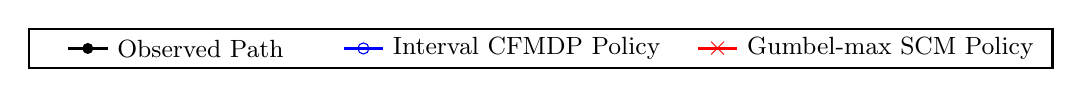
\begin{tikzpicture}[scale=1.0, every node/.style={scale=1.0}]
            \draw[thick, black] (-3, -0.25) rectangle (10, 0.25);
            %
            \draw[black, line width=1pt] (-2.5, 0.0) -- (-2,0.0);
            \fill[black] (-2.25,0.0) circle (2pt); %
            \node[right] at (-2,0.0) {\small Observed Path};
            
            %
            \draw[blue, line width=1pt] (1.0,0.0) -- (1.5,0.0);
            \node[draw=blue, circle, minimum size=4pt, inner sep=0pt] at (1.25,0.0) {}; %
            \node[right] at (1.5,0.0) {\small Interval CFMDP Policy};
            
            %
            \draw[red, line width=1pt] (5.5,0) -- (6,0);
            \node[red] at (5.75,0) {$\boldsymbol{\times}$}; %
            \node[right] at (6,0) {\small Gumbel-max SCM Policy};
        \end{tikzpicture}
    }\\
    %
    \subfigure[\footnotesize Lowest cumulative reward: Interval CFMDP ($312$), Gumbel-max SCM ($312$)]{%
        \resizebox{0.76\columnwidth}{!}{
             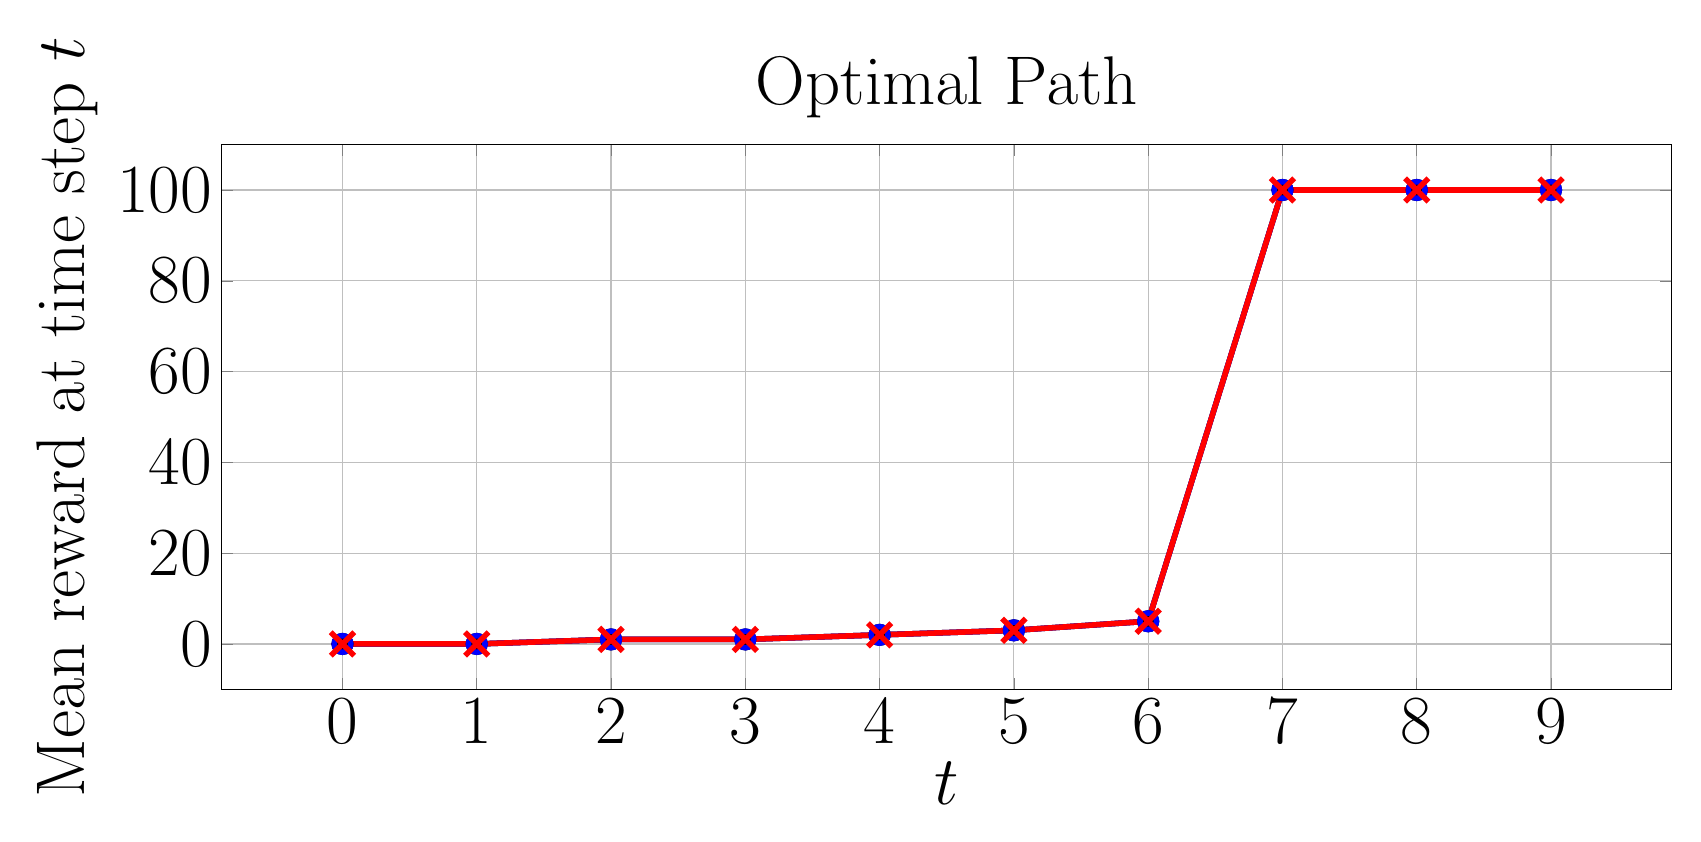
\begin{tikzpicture}
                \begin{axis}[
                    xlabel={$t$},
                    ylabel={Mean reward at time step $t$},
                    title={Optimal Path},
                    grid=both,
                    width=20cm, height=8.5cm,
                    every axis/.style={font=\Huge},
                    %
                ]
                \addplot[
                    color=black, %
                    mark=*, %
                    line width=2pt,
                    mark size=3pt,
                    error bars/.cd,
                    y dir=both, %
                    y explicit, %
                    error bar style={line width=1pt,solid},
                    error mark options={line width=1pt,mark size=4pt,rotate=90}
                ]
                coordinates {
                    (0, 0.0)  +- (0, 0.0)
                    (1, 0.0)  +- (0, 0.0) 
                    (2, 1.0)  +- (0, 0.0) 
                    (3, 1.0)  +- (0, 0.0)
                    (4, 2.0)  +- (0, 0.0)
                    (5, 3.0) +- (0, 0.0)
                    (6, 5.0) +- (0, 0.0)
                    (7, 100.0) +- (0, 0.0)
                    (8, 100.0) +- (0, 0.0)
                    (9, 100.0) +- (0, 0.0)
                };
                %
                \addplot[
                    color=blue, %
                    mark=o, %
                    line width=2pt,
                    mark size=3pt,
                    error bars/.cd,
                    y dir=both, %
                    y explicit, %
                    error bar style={line width=1pt,solid},
                    error mark options={line width=1pt,mark size=4pt,rotate=90}
                ]
                 coordinates {
                    (0, 0.0)  +- (0, 0.0)
                    (1, 0.0)  +- (0, 0.0) 
                    (2, 1.0)  +- (0, 0.0) 
                    (3, 1.0)  +- (0, 0.0)
                    (4, 2.0)  +- (0, 0.0)
                    (5, 3.0) +- (0, 0.0)
                    (6, 5.0) +- (0, 0.0)
                    (7, 100.0) +- (0, 0.0)
                    (8, 100.0) +- (0, 0.0)
                    (9, 100.0) +- (0, 0.0)
                };
                %
                \addplot[
                    color=red, %
                    mark=x, %
                    line width=2pt,
                    mark size=6pt,
                    error bars/.cd,
                    y dir=both, %
                    y explicit, %
                    error bar style={line width=1pt,solid},
                    error mark options={line width=1pt,mark size=4pt,rotate=90}
                ]
                coordinates {
                    (0, 0.0)  +- (0, 0.0)
                    (1, 0.0)  +- (0, 0.0) 
                    (2, 1.0)  +- (0, 0.0) 
                    (3, 1.0)  +- (0, 0.0)
                    (4, 2.0)  +- (0, 0.0)
                    (5, 3.0) +- (0, 0.0)
                    (6, 5.0) +- (0, 0.0)
                    (7, 100.0) +- (0, 0.0)
                    (8, 100.0) +- (0, 0.0)
                    (9, 100.0) +- (0, 0.0)
                };
                \end{axis}
            \end{tikzpicture}
         }
    }
    \hspace{1cm}
    \subfigure[\footnotesize Lowest cumulative reward: Interval CFMDP ($19$), Gumbel-max SCM ($-88$)]{%
         \resizebox{0.76\columnwidth}{!}{
            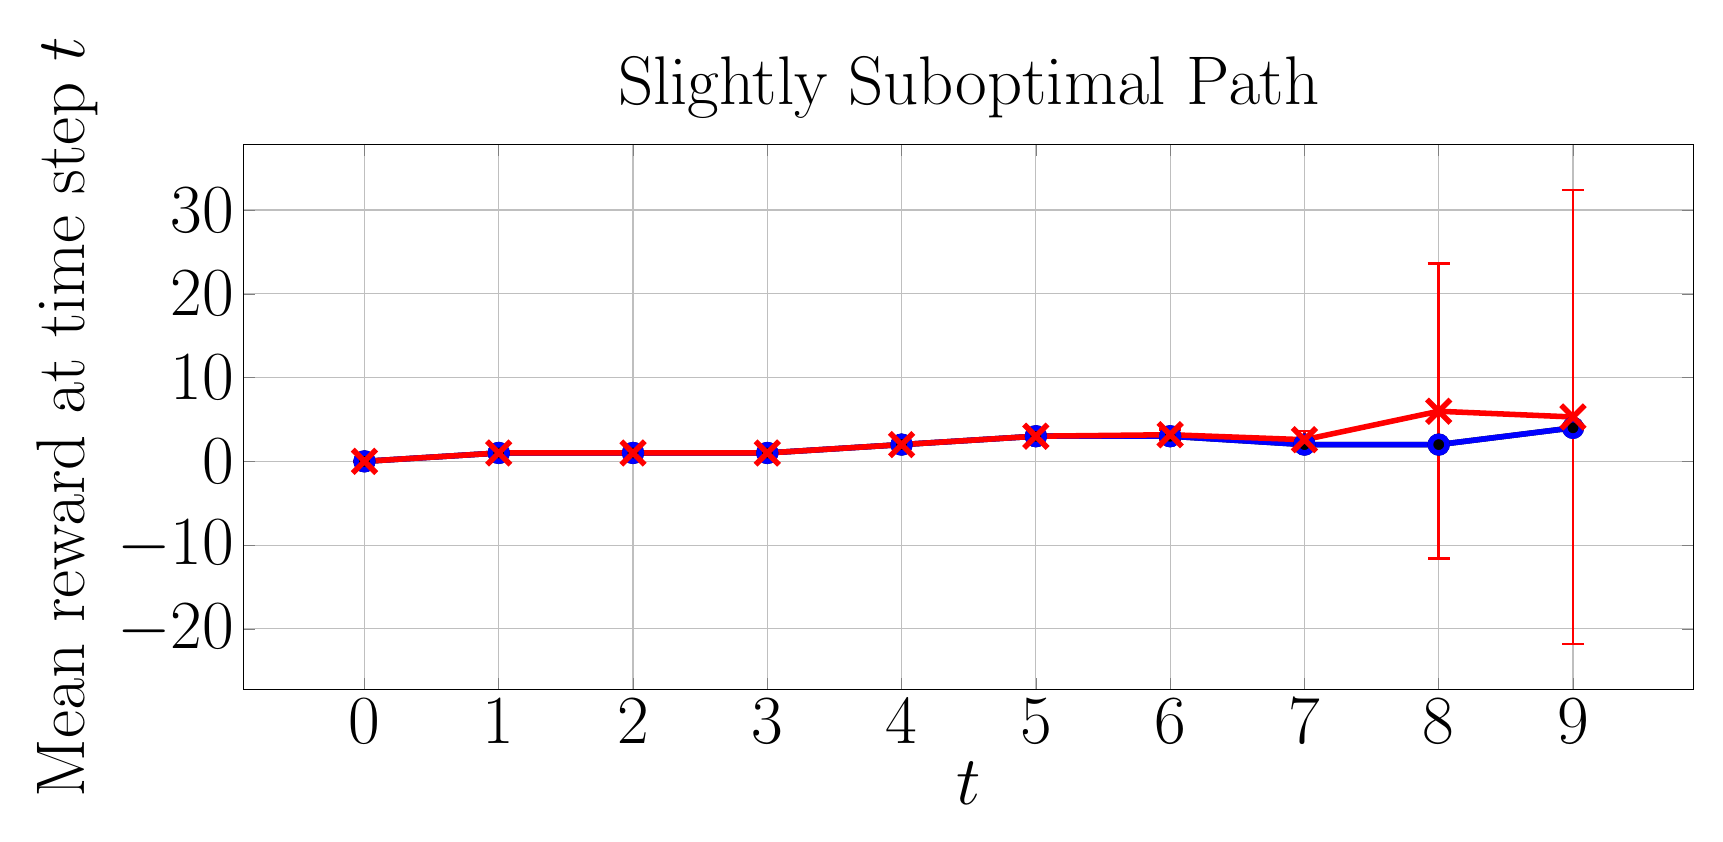
\begin{tikzpicture}
                \begin{axis}[
                    xlabel={$t$},
                    ylabel={Mean reward at time step $t$},
                    title={Slightly Suboptimal Path},
                    grid=both,
                    width=20cm, height=8.5cm,
                    every axis/.style={font=\Huge},
                    %
                ]
                \addplot[
                    color=black, %
                    mark=*, %
                    line width=2pt,
                    mark size=3pt,
                    error bars/.cd,
                    y dir=both, %
                    y explicit, %
                    error bar style={line width=1pt,solid},
                    error mark options={line width=1pt,mark size=4pt,rotate=90}
                ]
              coordinates {
                    (0, 0.0)  +- (0, 0.0)
                    (1, 1.0)  +- (0, 0.0) 
                    (2, 1.0)  +- (0, 0.0) 
                    (3, 1.0)  +- (0, 0.0)
                    (4, 2.0)  +- (0, 0.0)
                    (5, 3.0) +- (0, 0.0)
                    (6, 3.0) +- (0, 0.0)
                    (7, 2.0) +- (0, 0.0)
                    (8, 2.0) +- (0, 0.0)
                    (9, 4.0) +- (0, 0.0)
                };
                %
                \addplot[
                    color=blue, %
                    mark=o, %
                    line width=2pt,
                    mark size=3pt,
                    error bars/.cd,
                    y dir=both, %
                    y explicit, %
                    error bar style={line width=1pt,solid},
                    error mark options={line width=1pt,mark size=4pt,rotate=90}
                ]
              coordinates {
                    (0, 0.0)  +- (0, 0.0)
                    (1, 1.0)  +- (0, 0.0) 
                    (2, 1.0)  +- (0, 0.0) 
                    (3, 1.0)  +- (0, 0.0)
                    (4, 2.0)  +- (0, 0.0)
                    (5, 3.0) +- (0, 0.0)
                    (6, 3.0) +- (0, 0.0)
                    (7, 2.0) +- (0, 0.0)
                    (8, 2.0) +- (0, 0.0)
                    (9, 4.0) +- (0, 0.0)
                };
                %
                \addplot[
                    color=red, %
                    mark=x, %
                    line width=2pt,
                    mark size=6pt,
                    error bars/.cd,
                    y dir=both, %
                    y explicit, %
                    error bar style={line width=1pt,solid},
                    error mark options={line width=1pt,mark size=4pt,rotate=90}
                ]
                coordinates {
                    (0, 0.0)  +- (0, 0.0)
                    (1, 1.0)  +- (0, 0.0) 
                    (2, 1.0)  +- (0, 0.0) 
                    (3, 1.0)  +- (0, 0.0)
                    (4, 2.0)  += (0, 0.0)
                    (5, 3.0)  += (0, 0.0)
                    (6, 3.17847) += (0, 0.62606746) -= (0, 0.62606746)
                    (7, 2.5832885) += (0, 1.04598233) -= (0, 1.04598233)
                    (8, 5.978909) += (0, 17.60137623) -= (0, 17.60137623)
                    (9, 5.297059) += (0, 27.09227512) -= (0, 27.09227512)
                };
                \end{axis}
            \end{tikzpicture}
         }
    }\\[-1.5pt]
    \subfigure[\footnotesize Lowest cumulative reward: Interval CFMDP ($14$), Gumbel-max SCM ($-598$)]{%
         \resizebox{0.76\columnwidth}{!}{
             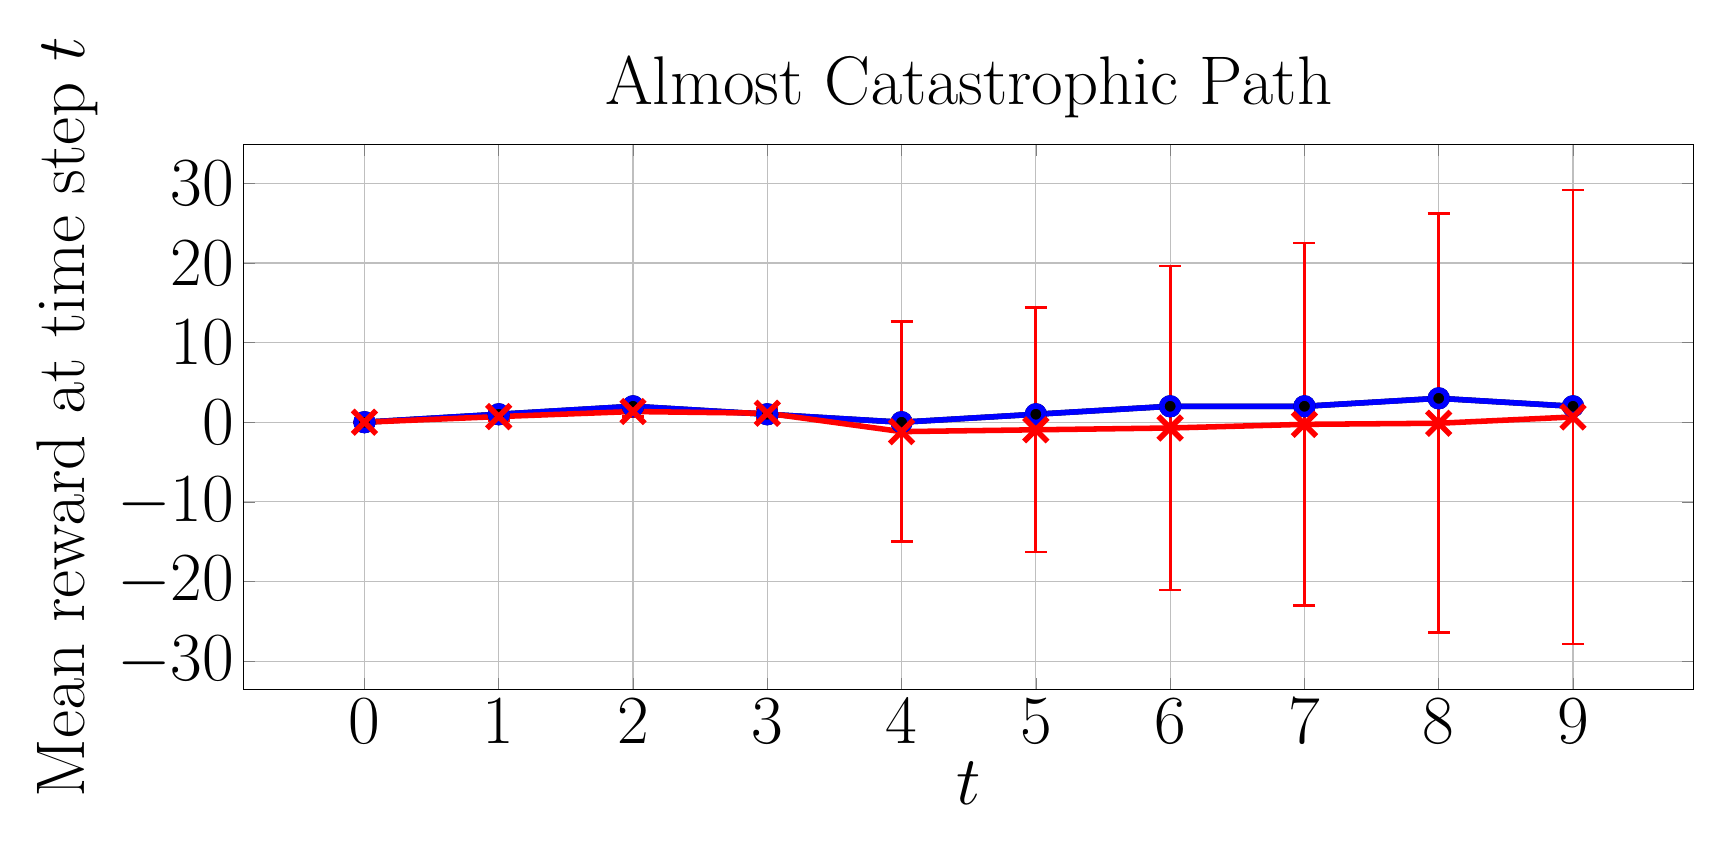
\begin{tikzpicture}
                \begin{axis}[
                    xlabel={$t$},
                    ylabel={Mean reward at time step $t$},
                    title={Almost Catastrophic Path},
                    grid=both,
                    width=20cm, height=8.5cm,
                    every axis/.style={font=\Huge},
                    %
                ]
                \addplot[
                    color=black, %
                    mark=*, %
                    line width=2pt,
                    mark size=3pt,
                    error bars/.cd,
                    y dir=both, %
                    y explicit, %
                    error bar style={line width=1pt,solid},
                    error mark options={line width=1pt,mark size=4pt,rotate=90}
                ]
                coordinates {
                    (0, 0.0)  +- (0, 0.0)
                    (1, 1.0)  +- (0, 0.0) 
                    (2, 2.0)  +- (0, 0.0) 
                    (3, 1.0)  +- (0, 0.0)
                    (4, 0.0)  +- (0, 0.0)
                    (5, 1.0) +- (0, 0.0)
                    (6, 2.0) +- (0, 0.0)
                    (7, 2.0) +- (0, 0.0)
                    (8, 3.0) +- (0, 0.0)
                    (9, 2.0) +- (0, 0.0)
                };
                %
                \addplot[
                    color=blue, %
                    mark=o, %
                    line width=2pt,
                    mark size=3pt,
                    error bars/.cd,
                    y dir=both, %
                    y explicit, %
                    error bar style={line width=1pt,solid},
                    error mark options={line width=1pt,mark size=4pt,rotate=90}
                ]
                coordinates {
                    (0, 0.0)  +- (0, 0.0)
                    (1, 1.0)  +- (0, 0.0) 
                    (2, 2.0)  +- (0, 0.0) 
                    (3, 1.0)  +- (0, 0.0)
                    (4, 0.0)  +- (0, 0.0)
                    (5, 1.0) +- (0, 0.0)
                    (6, 2.0) +- (0, 0.0)
                    (7, 2.0) +- (0, 0.0)
                    (8, 3.0) +- (0, 0.0)
                    (9, 2.0) +- (0, 0.0)
                };
                %
                \addplot[
                    color=red, %
                    mark=x, %
                    line width=2pt,
                    mark size=6pt,
                    error bars/.cd,
                    y dir=both, %
                    y explicit, %
                    error bar style={line width=1pt,solid},
                    error mark options={line width=1pt,mark size=4pt,rotate=90}
                ]
                coordinates {
                    (0, 0.0)  +- (0, 0.0)
                    (1, 0.7065655)  +- (0, 0.4553358) 
                    (2, 1.341673)  +- (0, 0.67091621) 
                    (3, 1.122926)  +- (0, 0.61281824)
                    (4, -1.1821935)  +- (0, 13.82444042)
                    (5, -0.952399)  +- (0, 15.35195457)
                    (6, -0.72672) +- (0, 20.33508414)
                    (7, -0.268983) +- (0, 22.77861454)
                    (8, -0.1310835) +- (0, 26.31013314)
                    (9, 0.65806) +- (0, 28.50670214)
                };
                %
            %
            %
            %
            %
            %
            %
            %
            %
            %
            %
            %
            %
            %
            %
            %
            %
            %
            %
                \end{axis}
            \end{tikzpicture}
         }
    }
    \hspace{1cm}
    \subfigure[\footnotesize Lowest cumulative reward: Interval CFMDP ($-698$), Gumbel-max SCM ($-698$)]{%
         \resizebox{0.76\columnwidth}{!}{
            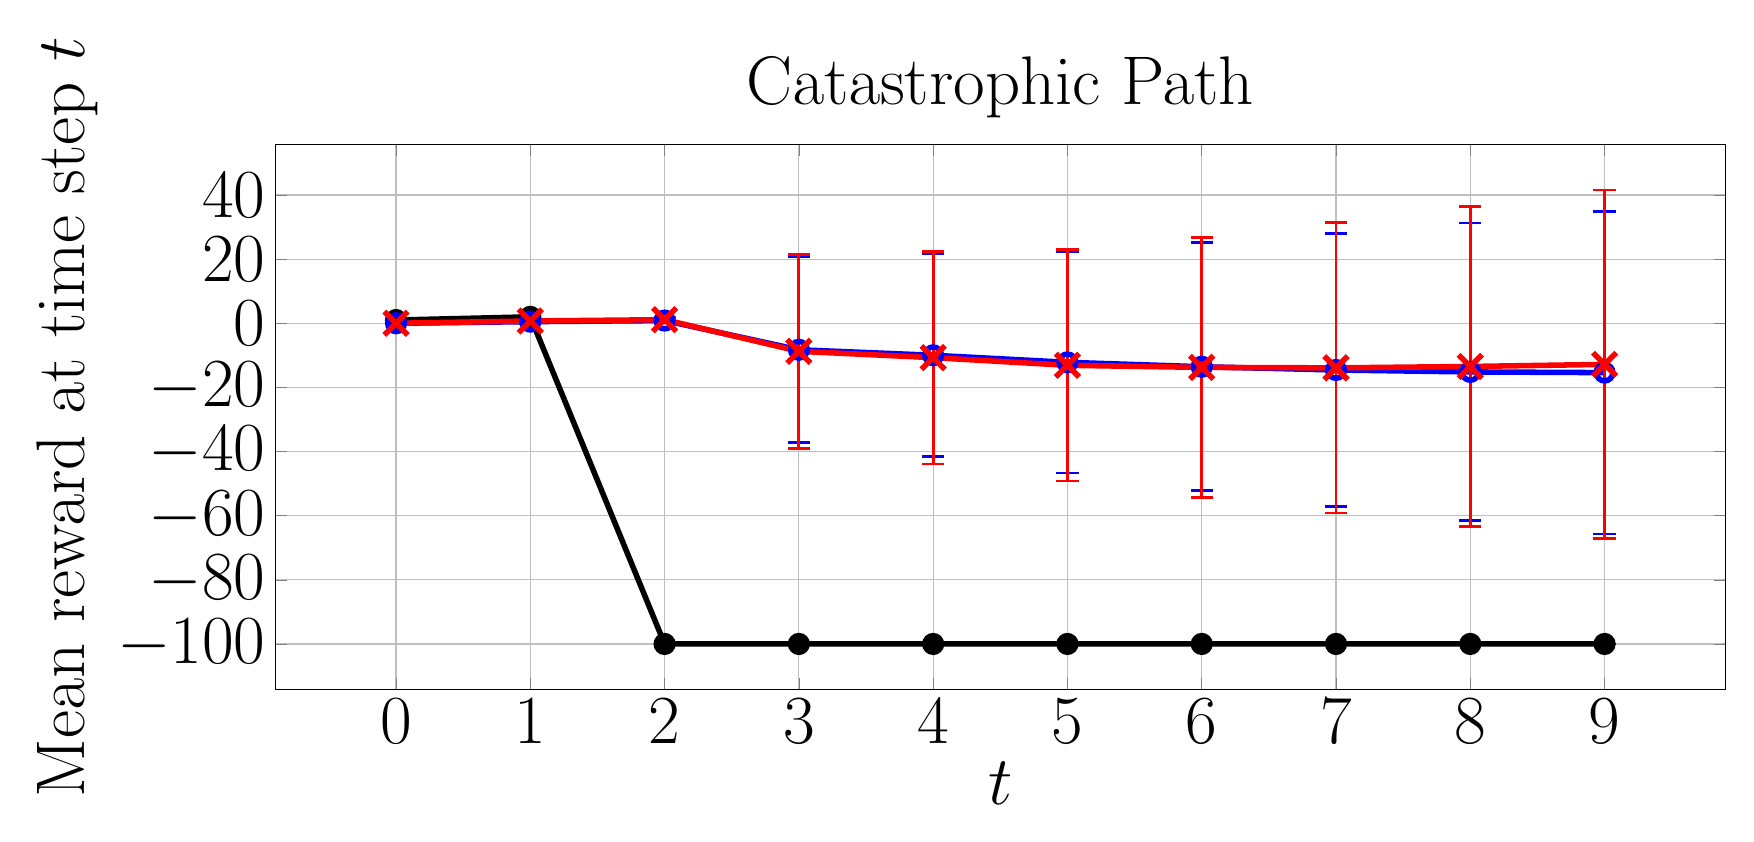
\begin{tikzpicture}
                \begin{axis}[
                    xlabel={$t$},
                    ylabel={Mean reward at time step $t$},
                    title={Catastrophic Path},
                    grid=both,
                    width=20cm, height=8.5cm,
                    every axis/.style={font=\Huge},
                    %
                ]
                \addplot[
                    color=black, %
                    mark=*, %
                    line width=2pt,
                    mark size=3pt,
                    error bars/.cd,
                    y dir=both, %
                    y explicit, %
                    error bar style={line width=1pt,solid},
                    error mark options={line width=1pt,mark size=4pt,rotate=90}
                ]
                coordinates {
                    (0, 1.0)  +- (0, 0.0)
                    (1, 2.0)  +- (0, 0.0) 
                    (2, -100.0)  +- (0, 0.0) 
                    (3, -100.0)  +- (0, 0.0)
                    (4, -100.0)  +- (0, 0.0)
                    (5, -100.0) +- (0, 0.0)
                    (6, -100.0) +- (0, 0.0)
                    (7, -100.0) +- (0, 0.0)
                    (8, -100.0) +- (0, 0.0)
                    (9, -100.0) +- (0, 0.0)
                };
                %
                \addplot[
                    color=blue, %
                    mark=o, %
                    line width=2pt,
                    mark size=3pt,
                    error bars/.cd,
                    y dir=both, %
                    y explicit, %
                    error bar style={line width=1pt,solid},
                    error mark options={line width=1pt,mark size=4pt,rotate=90}
                ]
                coordinates {
                    (0, 0.0)  +- (0, 0.0)
                    (1, 0.504814)  +- (0, 0.49997682) 
                    (2, 0.8439835)  +- (0, 0.76831917) 
                    (3, -8.2709165)  +- (0, 28.93656754)
                    (4, -9.981082)  +- (0, 31.66825363)
                    (5, -12.1776325) +- (0, 34.53463233)
                    (6, -13.556076) +- (0, 38.62845372)
                    (7, -14.574418) +- (0, 42.49603359)
                    (8, -15.1757075) +- (0, 46.41913968)
                    (9, -15.3900395) +- (0, 50.33563368)
                };
                %
                \addplot[
                    color=red, %
                    mark=x, %
                    line width=2pt,
                    mark size=6pt,
                    error bars/.cd,
                    y dir=both, %
                    y explicit, %
                    error bar style={line width=1pt,solid},
                    error mark options={line width=1pt,mark size=4pt,rotate=90}
                ]
                coordinates {
                    (0, 0.0)  +- (0, 0.0)
                    (1, 0.701873)  +- (0, 0.45743556) 
                    (2, 1.1227805)  +- (0, 0.73433129) 
                    (3, -8.7503255)  +- (0, 30.30257976)
                    (4, -10.722092)  +- (0, 33.17618589)
                    (5, -13.10721)  +- (0, 36.0648089)
                    (6, -13.7631645) +- (0, 40.56553451)
                    (7, -13.909043) +- (0, 45.23829402)
                    (8, -13.472517) +- (0, 49.96270296)
                    (9, -12.8278835) +- (0, 54.38618735)
                };
                %
            %
            %
            %
            %
            %
            %
            %
            %
            %
            %
            %
            %
            %
            %
            %
            %
            %
            %
                \end{axis}
            \end{tikzpicture}
         }
    }
    \caption{Average instant reward of CF paths induced by policies on GridWorld $p=0.4$.}
    \label{fig: reward p=0.4}
\end{figure*}

\subsection{Experimental Setup}
To compare policy performance, we measure the average rewards of counterfactual paths induced by our policy and the Gumbel-max policy by uniformly sampling $200$ counterfactual MDPs from the ICFMDP and generating $10,000$ counterfactual paths over each sampled CFMDP. \jl{Since the interval CFMDP depends on the observed path, we select $4$  paths of varying optimality to evaluate how the observed path impacts the performance of both policies: an optimal path, a slightly suboptimal path that could reach the optimal reward with a few changes, a catastrophic path that enters a catastrophic, terminal state with low reward, and an almost catastrophic path that was close to entering a catastrophic state.} When measuring the average probability bound widths and execution time needed to generate the ICFMDPs, we averaged over $20$ randomly generated observed paths
\footnote{Further training details are provided in Appendix \ref{app: training details}, and the code is provided at \href{https://github.com/ddv-lab/robust-cf-inference-in-MDPs}{https://github.com/ddv-lab/robust-cf-inference-in-MDPs}
%
%
.}.

\subsection{GridWorld}
\jl{The GridWorld MDP is a $4 \times 4$ grid where an agent must navigate from the top-left corner to the goal state in the bottom-right corner, avoiding a dangerous terminal state in the centre. At each time step, the agent can move up, down, left, or right, but there is a small probability (controlled by hyper-parameter $p$) of moving in an unintended direction. As the agent nears the goal, the reward for each state increases, culminating in a reward of $+100$ for reaching the goal. Entering the dangerous state results in a penalty of $-100$. We use two versions of GridWorld: a less stochastic version with $p=0.9$ (i.e., $90$\% chance of moving in the chosen direction) and a more stochastic version with $p=0.4$.}

\paragraph{GridWorld ($p=0.9$)}
When $p=0.9$, the counterfactual probability bounds are typically narrow (see Table \ref{tab:nonzero_probs} for average measurements). Consequently, as shown in Figure \ref{fig: reward p=0.9}, both policies are nearly identical and perform similarly well across the optimal, slightly suboptimal, and catastrophic paths.
%
However, for the almost catastrophic path, the interval CFMDP path is more conservative and follows the observed path more closely (as this is where the probability bounds are narrowest), which typically requires one additional step to reach the goal state than the Gumbel-max SCM policy.
%

\paragraph{GridWorld ($p=0.4$)}
\jl{When $p=0.4$, the GridWorld environment becomes more uncertain, increasing the risk of entering the dangerous state even if correct actions are chosen. Thus, as shown in Figure \ref{fig: reward p=0.4}, the interval CFMDP policy adopts a more conservative approach, avoiding deviation from the observed policy if it cannot guarantee higher counterfactual rewards (see the slightly suboptimal and almost catastrophic paths), whereas the Gumbel-max SCM is inconsistent: it can yield higher rewards, but also much lower rewards, reflected in the wide error bars.} For the catastrophic path, both policies must deviate from the observed path to achieve a higher reward and, in this case, perform similarly.
%
%
%
%
\subsection{Sepsis}
The Sepsis MDP \citep{oberst2019counterfactual} simulates trajectories of Sepsis patients. Each state consists of four vital signs (heart rate, blood pressure, oxygen concentration, and glucose levels), categorised as low, normal, or high.
and three treatments that can be toggled on/off at each time step (8 actions in total). Unlike \citet{oberst2019counterfactual}, we scale rewards based on the number of out-of-range vital signs, between $-1000$ (patient dies) and $1000$ (patient discharged). \jl{Like the GridWorld $p=0.4$ experiment, the Sepsis MDP is highly uncertain, as many states are equally likely to lead to optimal and poor outcomes. Thus, as shown in Figure \ref{fig: reward sepsis}, both policies follow the observed optimal and almost catastrophic paths to guarantee rewards are no worse than the observation.} However, improving the catastrophic path requires deviating from the observation. Here, the Gumbel-max SCM policy, on average, performs better than the interval CFMDP policy. But, since both policies have lower bounds clipped at $-1000$, neither policy reliably improves over the observation. In contrast, for the slightly suboptimal path, the interval CFMDP policy performs significantly better, shown by its higher lower bounds. 
Moreover, in these two cases, the worst-case counterfactual path generated by the interval CFMDP policy is better than that of the Gumbel-max SCM policy,
indicating its greater robustness.
%
\begin{figure*}
    \centering
     \resizebox{0.6\textwidth}{!}{
        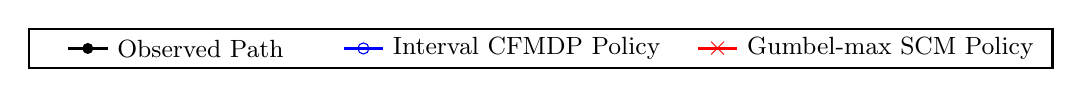
\begin{tikzpicture}[scale=1.0, every node/.style={scale=1.0}]
            \draw[thick, black] (-3, -0.25) rectangle (10, 0.25);
            %
            \draw[black, line width=1pt] (-2.5, 0.0) -- (-2,0.0);
            \fill[black] (-2.25,0.0) circle (2pt); %
            \node[right] at (-2,0.0) {\small Observed Path};
            
            %
            \draw[blue, line width=1pt] (1.0,0.0) -- (1.5,0.0);
            \node[draw=blue, circle, minimum size=4pt, inner sep=0pt] at (1.25,0.0) {}; %
            \node[right] at (1.5,0.0) {\small Interval CFMDP Policy};
            
            %
            \draw[red, line width=1pt] (5.5,0) -- (6,0);
            \node[red] at (5.75,0) {$\boldsymbol{\times}$}; %
            \node[right] at (6,0) {\small Gumbel-max SCM Policy};
        \end{tikzpicture}
    }\\
    \subfigure[\footnotesize Lowest cumulative reward: Interval CFMDP ($8000$), Gumbel-max SCM ($8000$)]{%
         \resizebox{0.76\columnwidth}{!}{
             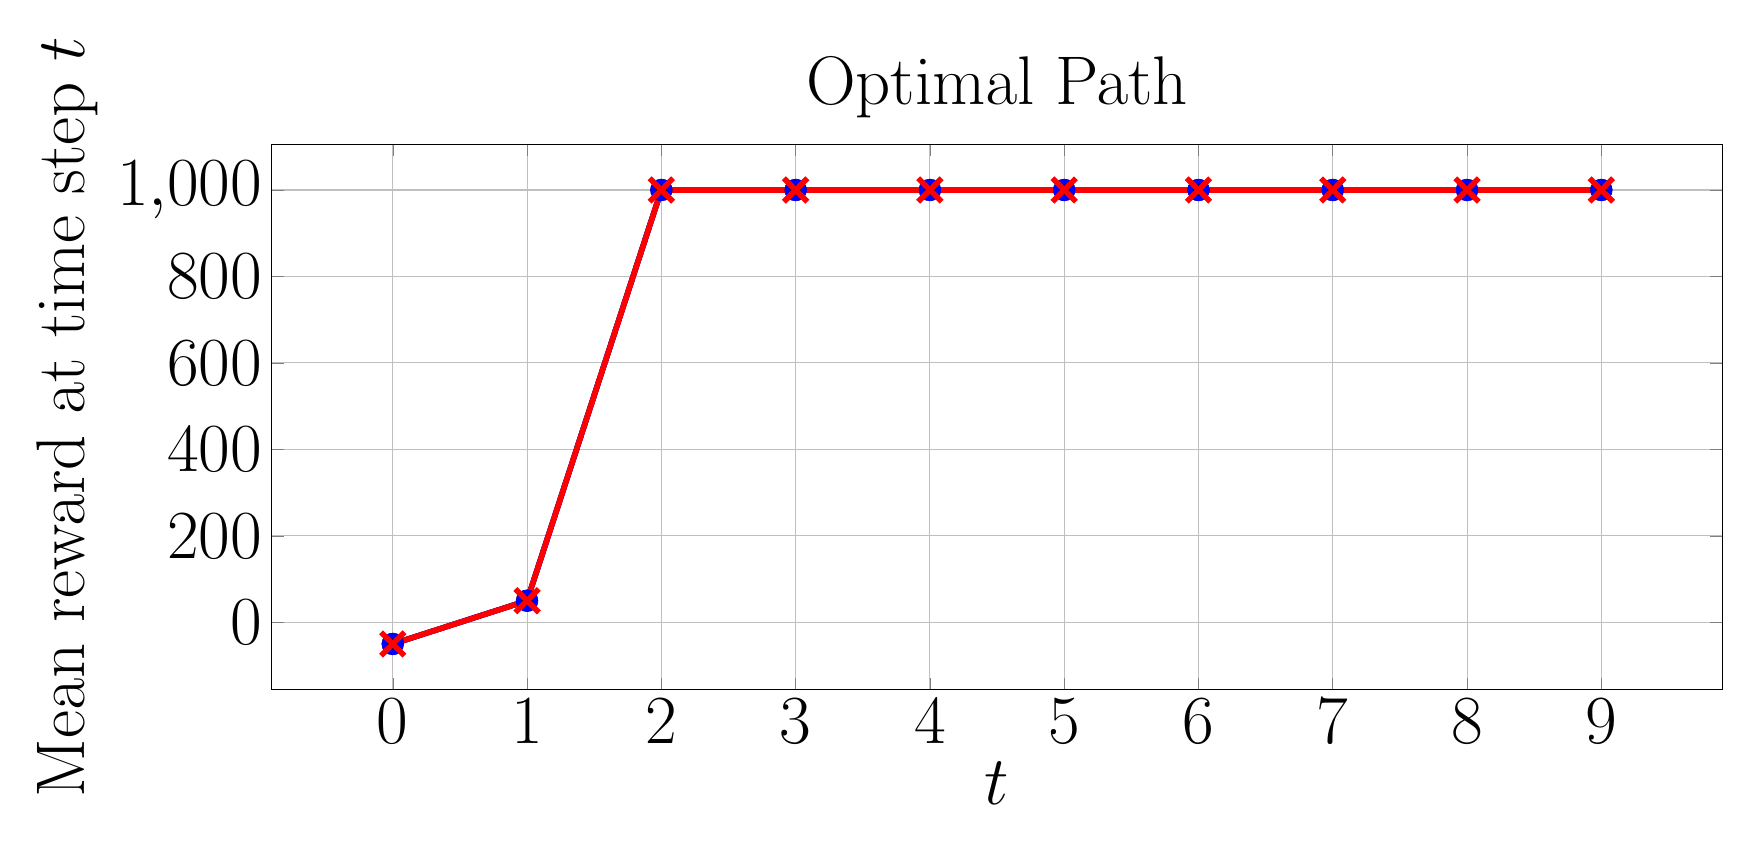
\begin{tikzpicture}
                \begin{axis}[
                    xlabel={$t$},
                    ylabel={Mean reward at time step $t$},
                    title={Optimal Path},
                    grid=both,
                    width=20cm, height=8.5cm,
                    every axis/.style={font=\Huge},
                    %
                ]
                \addplot[
                    color=black, %
                    mark=*, %
                    line width=2pt,
                    mark size=3pt,
                ]
                coordinates {
                    (0, -50.0)
                    (1, 50.0)
                    (2, 1000.0)
                    (3, 1000.0)
                    (4, 1000.0)
                    (5, 1000.0)
                    (6, 1000.0)
                    (7, 1000.0)
                    (8, 1000.0)
                    (9, 1000.0)
                };
                %
                \addplot[
                    color=blue, %
                    mark=o, %
                    line width=2pt,
                    mark size=3pt,
                    error bars/.cd,
                    y dir=both, %
                    y explicit, %
                    error bar style={line width=1pt,solid},
                    error mark options={line width=1pt,mark size=4pt,rotate=90}
                ]
                coordinates {
                    (0, -50.0)  +- (0, 0.0)
                    (1, 50.0)  +- (0, 0.0) 
                    (2, 1000.0)  +- (0, 0.0) 
                    (3, 1000.0)  +- (0, 0.0)
                    (4, 1000.0)  +- (0, 0.0)
                    (5, 1000.0) +- (0, 0.0)
                    (6, 1000.0) +- (0, 0.0)
                    (7, 1000.0) +- (0, 0.0)
                    (8, 1000.0) +- (0, 0.0)
                    (9, 1000.0) +- (0, 0.0)
                };
                %
                \addplot[
                    color=red, %
                    mark=x, %
                    line width=2pt,
                    mark size=6pt,
                    error bars/.cd,
                    y dir=both, %
                    y explicit, %
                    error bar style={line width=1pt,solid},
                    error mark options={line width=1pt,mark size=4pt,rotate=90}
                ]
                coordinates {
                    (0, -50.0)  +- (0, 0.0)
                    (1, 50.0)  +- (0, 0.0) 
                    (2, 1000.0)  +- (0, 0.0) 
                    (3, 1000.0)  +- (0, 0.0)
                    (4, 1000.0)  +- (0, 0.0)
                    (5, 1000.0) +- (0, 0.0)
                    (6, 1000.0) +- (0, 0.0)
                    (7, 1000.0) +- (0, 0.0)
                    (8, 1000.0) +- (0, 0.0)
                    (9, 1000.0) +- (0, 0.0)
                };
                %
                \end{axis}
            \end{tikzpicture}
         }
    }
    \hspace{1cm}
    \subfigure[\footnotesize Lowest cumulative reward: Interval CFMDP ($-5980$), Gumbel-max SCM ($-8000$)]{%
         \resizebox{0.76\columnwidth}{!}{
            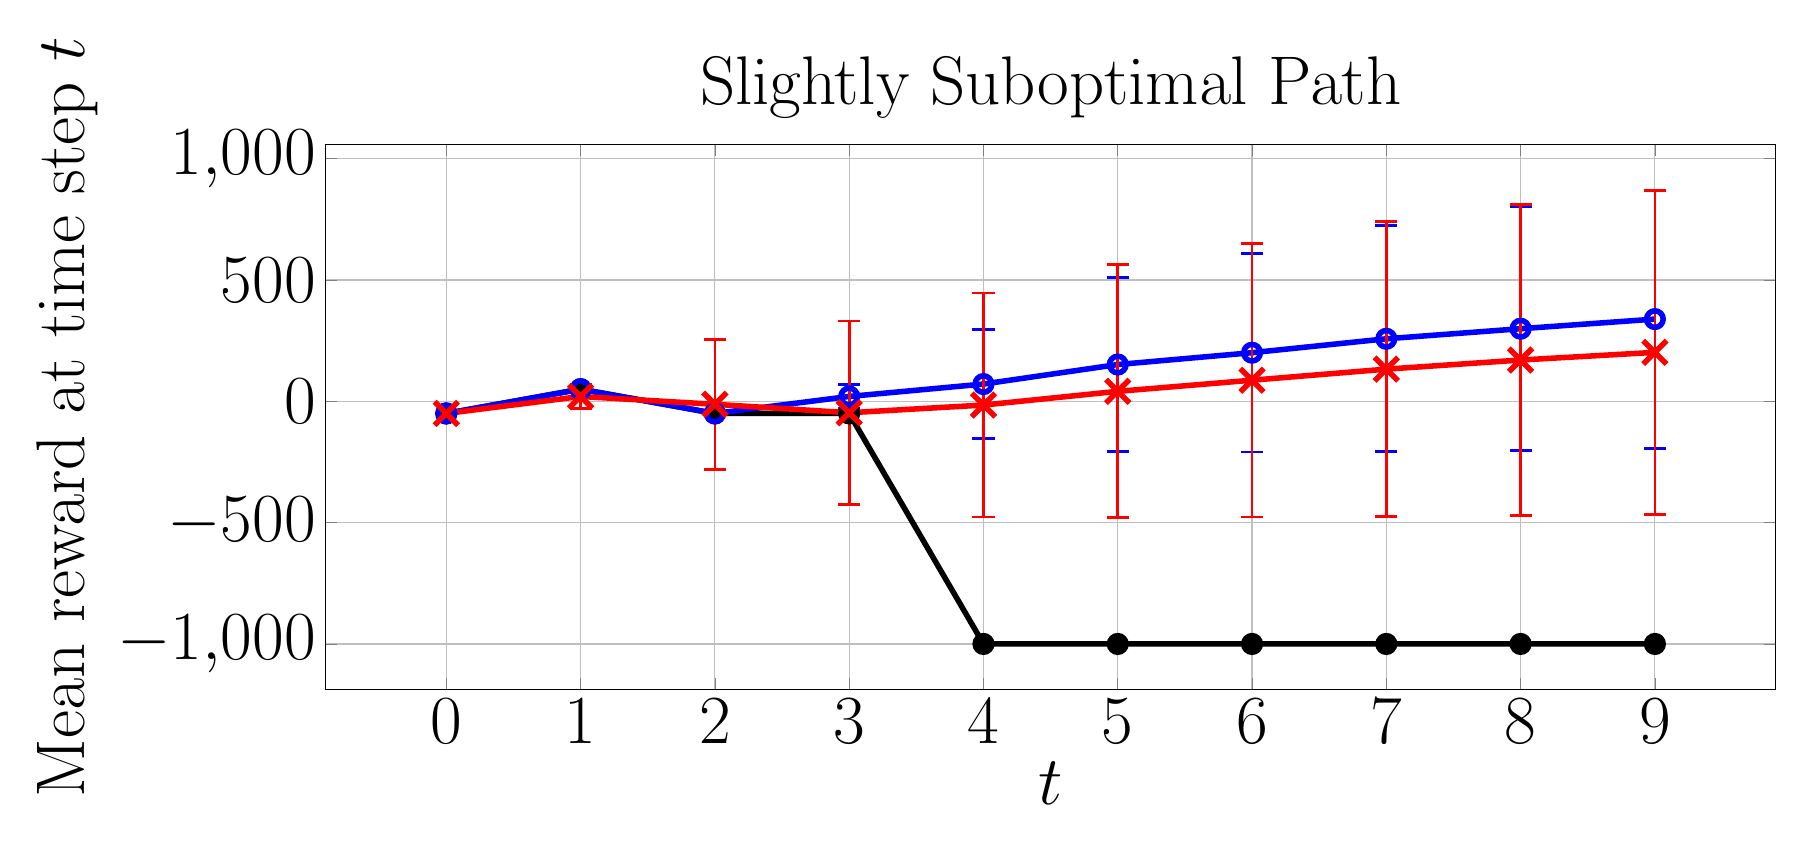
\begin{tikzpicture}
                \begin{axis}[
                    xlabel={$t$},
                    ylabel={Mean reward at time step $t$},
                    title={Slightly Suboptimal Path},
                    grid=both,
                    width=20cm, height=8.5cm,
                    every axis/.style={font=\Huge},
                    %
                ]
               \addplot[
                    color=black, %
                    mark=*, %
                    line width=2pt,
                    mark size=3pt,
                ]
                coordinates {
                    (0, -50.0)
                    (1, 50.0)
                    (2, -50.0)
                    (3, -50.0)
                    (4, -1000.0)
                    (5, -1000.0)
                    (6, -1000.0)
                    (7, -1000.0)
                    (8, -1000.0)
                    (9, -1000.0)
                };
                %
                \addplot[
                    color=blue, %
                    mark=o, %
                    line width=2pt,
                    mark size=3pt,
                    error bars/.cd,
                    y dir=both, %
                    y explicit, %
                    error bar style={line width=1pt,solid},
                    error mark options={line width=1pt,mark size=4pt,rotate=90}
                ]
                coordinates {
                    (0, -50.0)  +- (0, 0.0)
                    (1, 50.0)  +- (0, 0.0) 
                    (2, -50.0)  +- (0, 0.0) 
                    (3, 20.0631)  +- (0, 49.97539413)
                    (4, 71.206585)  +- (0, 226.02033693)
                    (5, 151.60797) +- (0, 359.23292559)
                    (6, 200.40593) +- (0, 408.86185176)
                    (7, 257.77948) +- (0, 466.10372804)
                    (8, 299.237465) +- (0, 501.82579506)
                    (9, 338.9129) +- (0, 532.06124996)
                };
                %
                \addplot[
                    color=red, %
                    mark=x, %
                    line width=2pt,
                    mark size=6pt,
                    error bars/.cd,
                    y dir=both, %
                    y explicit, %
                    error bar style={line width=1pt,solid},
                    error mark options={line width=1pt,mark size=4pt,rotate=90}
                ]
                coordinates {
                    (0, -50.0)  +- (0, 0.0)
                    (1, 20.00736)  +- (0, 49.99786741) 
                    (2, -12.282865)  +- (0, 267.598755) 
                    (3, -47.125995)  +- (0, 378.41755832)
                    (4, -15.381965)  +- (0, 461.77616558)
                    (5, 41.15459) +- (0, 521.53189262)
                    (6, 87.01595) +- (0, 564.22243126 )
                    (7, 132.62376) +- (0, 607.31338037)
                    (8, 170.168145) +- (0, 641.48013693)
                    (9, 201.813135) +- (0, 667.29441777)
                };
                %
                %
                %
                %
                %
                %
                %
                %
                %
                %
                %
                %
                %
                %
                %
                %
                %
                %
                %
                \end{axis}
            \end{tikzpicture}
         }
    }\\[-1.5pt]
    \subfigure[\footnotesize Lowest cumulative reward: Interval CFMDP ($100$), Gumbel-max SCM ($100$)]{%
         \resizebox{0.76\columnwidth}{!}{
             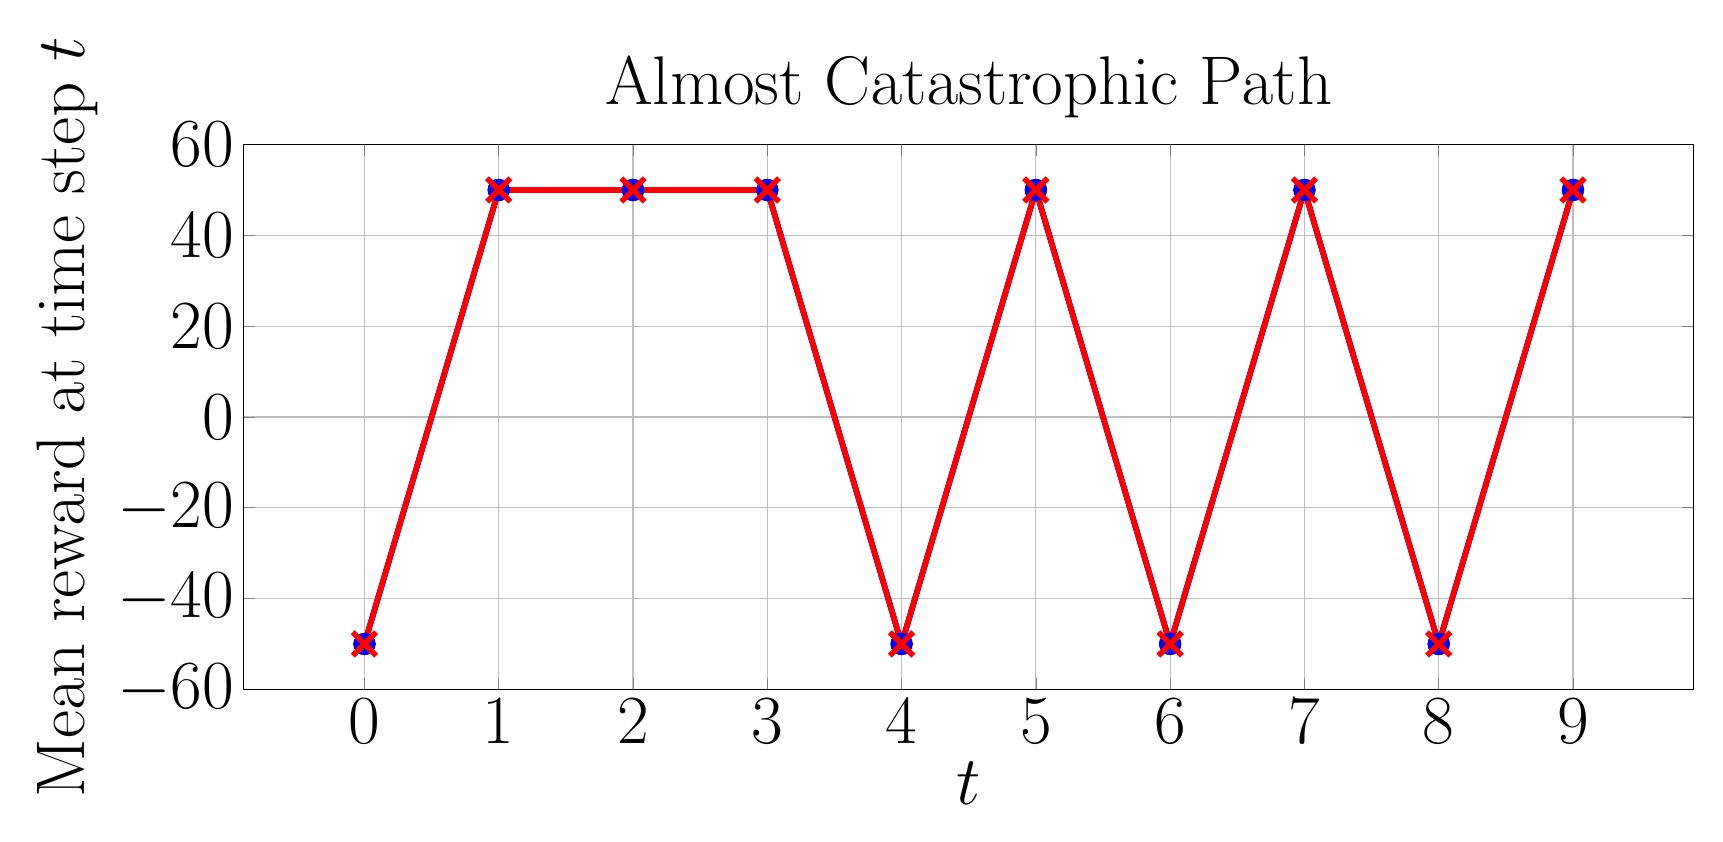
\begin{tikzpicture}
                \begin{axis}[
                    xlabel={$t$},
                    ylabel={Mean reward at time step $t$},
                    title={Almost Catastrophic Path},
                    grid=both,
                    every axis/.style={font=\Huge},
                    width=20cm, height=8.5cm,
                    %
                ]
               \addplot[
                    color=black, %
                    mark=*, %
                    line width=2pt,
                    mark size=3pt,
                ]
                coordinates {
                    (0, -50.0)
                    (1, 50.0)
                    (2, 50.0)
                    (3, 50.0)
                    (4, -50.0)
                    (5, 50.0)
                    (6, -50.0)
                    (7, 50.0)
                    (8, -50.0)
                    (9, 50.0)
                };
                %
                %
                \addplot[
                    color=blue, %
                    mark=o, %
                    line width=2pt,
                    mark size=3pt,
                    error bars/.cd,
                    y dir=both, %
                    y explicit, %
                    error bar style={line width=1pt,solid},
                    error mark options={line width=1pt,mark size=4pt,rotate=90}
                ]
                coordinates {
                    (0, -50.0)  +- (0, 0.0)
                    (1, 50.0)  +- (0, 0.0) 
                    (2, 50.0)  +- (0, 0.0) 
                    (3, 50.0)  +- (0, 0.0)
                    (4, -50.0)  +- (0, 0.0)
                    (5, 50.0) +- (0, 0.0)
                    (6, -50.0) +- (0, 0.0)
                    (7, 50.0) +- (0, 0.0)
                    (8, -50.0) +- (0, 0.0)
                    (9, 50.0) +- (0, 0.0)
                };
                %
                \addplot[
                    color=red, %
                    mark=x, %
                    line width=2pt,
                    mark size=6pt,
                    error bars/.cd,
                    y dir=both, %
                    y explicit, %
                    error bar style={line width=1pt,solid},
                    error mark options={line width=1pt,mark size=4pt,rotate=90}
                ]
                coordinates {
                    (0, -50.0)  +- (0, 0.0)
                    (1, 50.0)  +- (0, 0.0) 
                    (2, 50.0)  +- (0, 0.0) 
                    (3, 50.0)  +- (0, 0.0)
                    (4, -50.0)  +- (0, 0.0)
                    (5, 50.0) +- (0, 0.0)
                    (6, -50.0) +- (0, 0.0)
                    (7, 50.0) +- (0, 0.0)
                    (8, -50.0) +- (0, 0.0)
                    (9, 50.0) +- (0, 0.0)
                };
                %
                %
                %
                %
                %
                %
                %
                %
                %
                %
                %
                %
                %
                %
                %
                %
                %
                %
                %
                \end{axis}
            \end{tikzpicture}
         }
    }
    \hspace{1cm}
    \subfigure[\footnotesize Lowest cumulative reward: Interval CFMDP ($-7150$), Gumbel-max SCM ($-9050$)]{%
         \resizebox{0.76\columnwidth}{!}{
            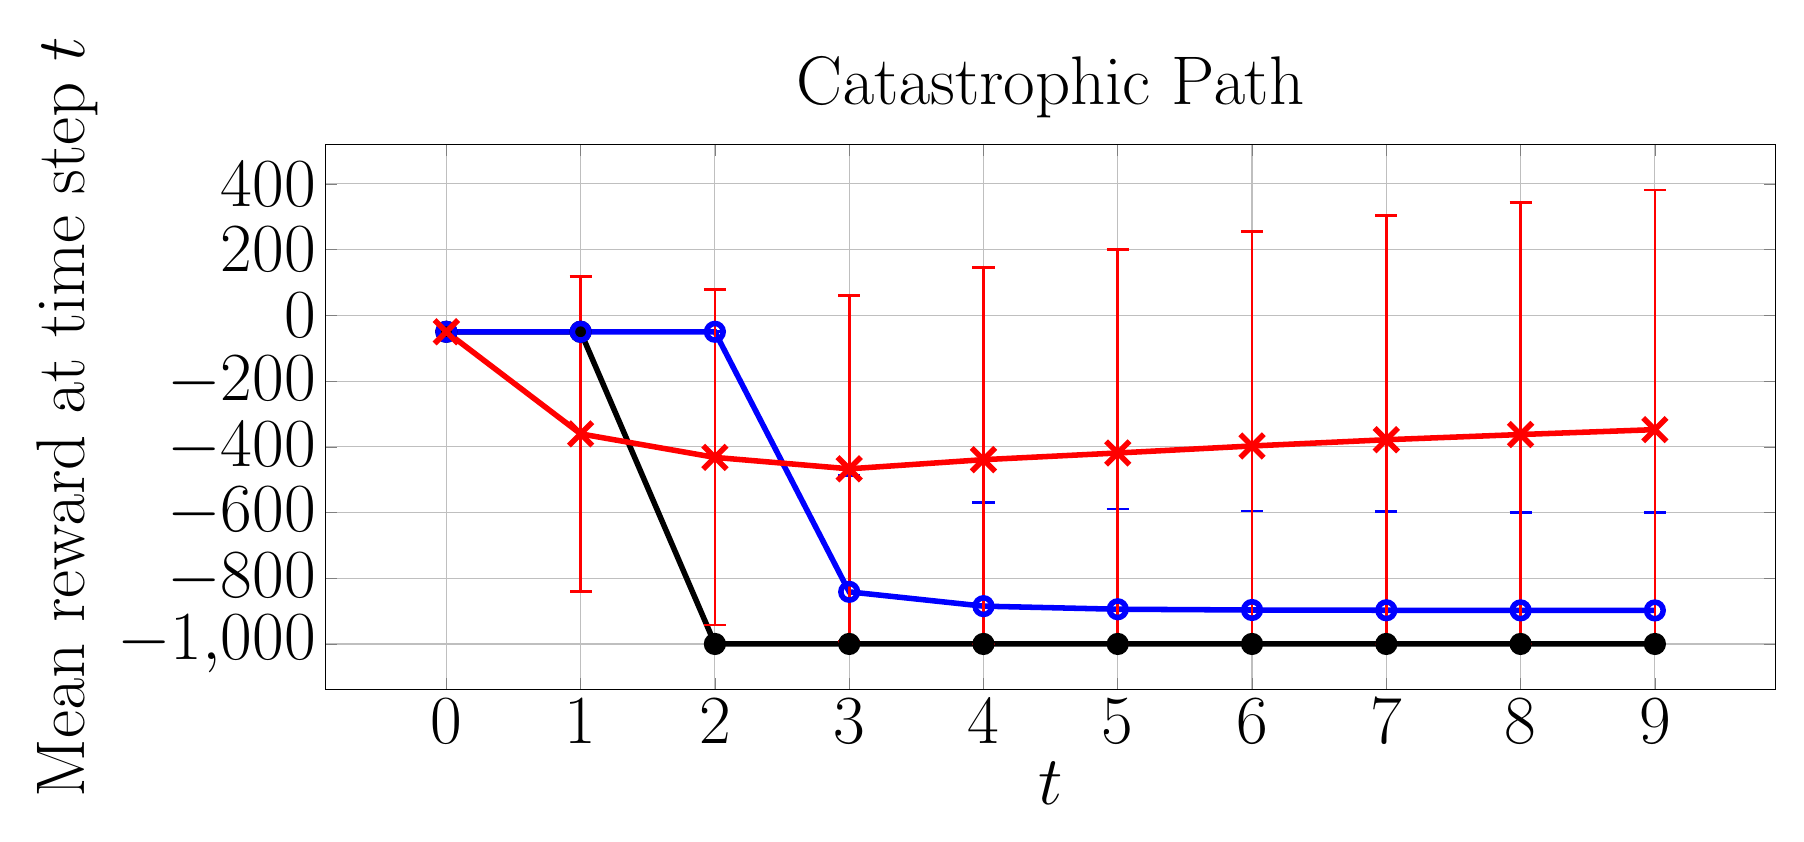
\begin{tikzpicture}
                \begin{axis}[
                    xlabel={$t$},
                    ylabel={Mean reward at time step $t$},
                    title={Catastrophic Path},
                    grid=both,
                    width=20cm, height=8.5cm,
                    every axis/.style={font=\Huge},
                    %
                ]
               \addplot[
                    color=black, %
                    mark=*, %
                    line width=2pt,
                    mark size=3pt,
                ]
                coordinates {
                    (0, -50.0)
                    (1, -50.0)
                    (2, -1000.0)
                    (3, -1000.0)
                    (4, -1000.0)
                    (5, -1000.0)
                    (6, -1000.0)
                    (7, -1000.0)
                    (8, -1000.0)
                    (9, -1000.0)
                };
                %
                %
                \addplot[
                    color=blue, %
                    mark=o, %
                    line width=2pt,
                    mark size=3pt,
                    error bars/.cd,
                    y dir=both, %
                    y explicit, %
                    error bar style={line width=1pt,solid},
                    error mark options={line width=1pt,mark size=4pt,rotate=90}
                ]
                coordinates {
                    (0, -50.0)  +- (0, 0.0)
                    (1, -50.0)  +- (0, 0.0) 
                    (2, -50.0)  +- (0, 0.0) 
                    (3, -841.440725)  += (0, 354.24605512) -= (0, 158.559275)
                    (4, -884.98225)  += (0, 315.37519669) -= (0, 115.01775)
                    (5, -894.330425) += (0, 304.88572805) -= (0, 105.669575)
                    (6, -896.696175) += (0, 301.19954514) -= (0, 103.303825)
                    (7, -897.4635) += (0, 299.61791279) -= (0, 102.5365)
                    (8, -897.77595) += (0, 298.80392585) -= (0, 102.22405)
                    (9, -897.942975) += (0, 298.32920557) -= (0, 102.057025)
                };
                %
                \addplot[
                    color=red, %
                    mark=x, %
                    line width=2pt,
                    mark size=6pt,
                    error bars/.cd,
                    y dir=both, %
                    y explicit, %
                    error bar style={line width=1pt,solid},
                    error mark options={line width=1pt,mark size=4pt,rotate=90}
                ]
            coordinates {
                    (0, -50.0)  +- (0, 0.0)
                    (1, -360.675265)  +- (0, 479.39812699) 
                    (2, -432.27629)  +- (0, 510.38620897) 
                    (3, -467.029545)  += (0, 526.36009628) -= (0, 526.36009628)
                    (4, -439.17429)  += (0, 583.96638919) -= (0, 560.82571)
                    (5, -418.82704) += (0, 618.43027478) -= (0, 581.17296)
                    (6, -397.464895) += (0, 652.67322574) -= (0, 602.535105)
                    (7, -378.49052) += (0, 682.85407033) -= (0, 621.50948)
                    (8, -362.654195) += (0, 707.01412023) -= (0, 637.345805)
                    (9, -347.737935) += (0, 729.29076479) -= (0, 652.262065)
                };
                %
                %
                %
                %
                %
                %
                %
                %
                %
                %
                %
                %
                %
                %
                %
                %
                %
                %
                %
                \end{axis}
            \end{tikzpicture}
         }
    }
    \caption{Average instant reward of CF paths induced by policies on Sepsis.}
    \label{fig: reward sepsis}
\end{figure*}

%
%
%
\subsection{Interval CFMDP Bounds}
%
%
Table \ref{tab:nonzero_probs} presents the mean counterfactual probability bound widths (excluding transitions where the upper bound is $0$) for each MDP, averaged over 20 observed paths. We compare the bounds under counterfactual stability (CS) and monotonicity (M) assumptions, CS alone, and no assumptions. This shows that the assumptions marginally reduce the bound widths, indicating the assumptions tighten the bounds without excluding too many causal models, as intended.
\renewcommand{\arraystretch}{1}

\begin{table}
\centering
\caption{Mean width of counterfactual probability bounds}
\resizebox{0.8\columnwidth}{!}{%
\begin{tabular}{|c|c|c|c|}
\hline
\multirow{2}{*}{\textbf{Environment}} & \multicolumn{3}{c|}{\textbf{Assumptions}} \\ \cline{2-4}
 & \textbf{CS + M} & \textbf{CS} & \textbf{None\tablefootnote{\jl{Equivalent to \citet{li2024probabilities}'s bounds (see Section \ref{sec: equivalence with Li}).}}} \\ \hline
\textbf{GridWorld} ($p=0.9$) & 0.0817 & 0.0977 & 0.100 \\ \hline
\textbf{GridWorld} ($p=0.4$) & 0.552  & 0.638  & 0.646 \\ \hline
\textbf{Sepsis} & 0.138 & 0.140 & 0.140 \\ \hline
\end{tabular}
}
\label{tab:nonzero_probs}
\end{table}


\subsection{Execution Times}
Table \ref{tab: times} compares the average time needed to generate the interval CFMDP vs.\ the Gumbel-max SCM CFMDP for 20 observations.
The GridWorld algorithms were run single-threaded, while the Sepsis experiments were run in parallel.
Generating the interval CFMDP is significantly faster as it uses exact analytical bounds, whereas the Gumbel-max CFMDP requires sampling from the Gumbel distribution to estimate counterfactual transition probabilities. \jl{Since constructing the counterfactual MDP models is the main bottleneck in both approaches, ours is more efficient overall and suitable for larger MDPs.}
\begin{table}
\centering
\caption{Mean execution time to generate CFMDPs}
\resizebox{0.99\columnwidth}{!}{%
\begin{tabular}{|c|c|c|}
\hline
\multirow{2}{*}{\textbf{Environment}} & \multicolumn{2}{c|}{\textbf{Mean Execution Time (s)}} \\ \cline{2-3} 
                                      & \textbf{Interval CFMDP} & \textbf{Gumbel-max CFMDP} \\ \hline
\textbf{GridWorld ($p=0.9$) }                  & 0.261                   & 56.1                      \\ \hline
\textbf{GridWorld ($p=0.4$)  }                 & 0.336                   & 54.5                      \\ \hline
\textbf{Sepsis}                                 & 688                     & 2940                      \\ \hline
\end{tabular}%
}
\label{tab: times}
\end{table}
